\documentclass[12pt,a4paper,twoside,openright]{report}
	\usepackage[hyphens,spaces,obeyspaces]{url}
	\usepackage[pdfborder={0 0 0}]{hyperref}    % turns references into hyperlinks
	\usepackage[margin=25mm]{geometry}  % adjusts page layout
	\usepackage{graphicx}  % allows inclusion of PDF, PNG and JPG images
	\usepackage{verbatim}
	\usepackage{import} %import proposal from another folder
	\usepackage{pdfpages}
	\usepackage{listings}
	\usepackage{upquote}
	\usepackage{nameref}
	\usepackage{tikz}
	\usepackage{color}
	\usepackage[framemethod=tikz]{mdframed}
	\usepackage{courier}
	\usepackage{caption}
	\usepackage{subcaption}
	\usepackage{float}
	\usepackage[style=ieee]{biblatex} 
	\addbibresource{refs.bib}

	\definecolor{airforceblue}{rgb}{0.36, 0.54, 0.70}
	\definecolor{greyish}{rgb}{0.35, 0.35, 0.35}
 
	\newcommand{\vcenteredinclude}[1]{\begingroup
	\setbox0=\hbox{\includegraphics[width=4cm]{#1}}%
	\parbox{\wd0}{\box0}\endgroup}

	\usetikzlibrary{positioning,fit,calc}

	\lstset{
	language=[Objective]Caml,
	showstringspaces=false,
	breaklines=true,
	basicstyle=\normalsize\ttfamily,                 % Code font, Examples: \footnotesize, \ttfamily
	keywordstyle=\color{greyish}\textbf,
	commentstyle=\color{airforceblue},
	frame=tb,
	captionpos=b
	}


	\newcommand\tab[1][1cm]{\hspace*{#1}}
	\raggedbottom                           % try to  avoid widows and orphans
	\sloppy
	\clubpenalty1000%
	\widowpenalty1000%
	
	\renewcommand{\baselinestretch}{1.1}  

	\begin{document}

	\pagestyle{empty}
	
	\rightline{\LARGE \textbf{Charlie Crisp}}
	
	\vspace*{60mm}
	\begin{center}
	\Huge
	\textbf{Building a Blockchain Library for OCaml} \\[5mm]
	Computer Science Tripos -- Part II \\[5mm]
	Pembroke College \\[5mm]
	\today  % today's date
	\end{center}
	
	%%%%%%%%%%%%%%%%%%%%%%%%%%%%%%%%%%%%%%%%%%%%%%%%%%%%%%%%%%%%%%%%%%%%%%%%%%%%%%
	% Proforma, table of contents and list of figures
	
	\pagestyle{plain}
	
	\chapter*{Proforma}
	
	{\large
	\begin{tabular}{ll}
	Name:               & \bf Charlie Crisp                       \\
	College:            & \bf Pembroke College                     \\
	Project Title:      & \bf Building a Blockchain Library for OCaml \\
	Examination:        & \bf Computer Science Tripos -- Part II, July 2018  \\
	Word Count:         & \bf 11705\\
	Project Originator: & KC Sivaramakrishnan                    \\
	Supervisor:         & KC Sivaramakrishnan                    
	\end{tabular}
	}
	\stepcounter{footnote}
	
	
	\section*{Original Aims of the Project}
	
	The original aim of the project was to build a library in OCaml, which could be used as a building block for blockchain applications. 
	The library should allow participating nodes to own a shared copy of a blockchain data structure, agreed upon by all participating nodes.
	Nodes should also be able to commit transactions to the blockchain, which should then be visible to other participating nodes. 
	
	\section*{Work Completed}
	
	I have successfully built Logan, a blockchain library in OCaml.
	Logan achieves consensus using a simple leader based protocol where a leader will poll participants for new updates to add to the blockchain.
	Logan also provides the capability to run passive replicas which store the leader's state to allow full recovery in the even of a leader failure.
	Logan can achieve latencies of around 10 seconds and throughputs of up to 30 transactions per second. 
	Logan achieves many but not all of its success criteria however in this report I attribute the unfulfilled criteria to the implementation of Git used, rather than Logan's implementation.
	
	\section*{Special Difficulties}
	
	None
	
	\newpage
	\section*{Declaration}
	
	I, Charlie Crisp of Pembroke College, being a candidate for Part II of the Computer
	Science Tripos, hereby declare that this dissertation and the work described in it are my own work,
	unaided except as may be specified below, and that the dissertation
	does not contain material that has already been used to any substantial
	extent for a comparable purpose.
	
	\bigskip
	\noindent 
	Signed:
	\vcenteredinclude{figs/signature.png} \\ \\
	\bigskip
	\noindent 
	Date: \space \space \space \today
	
	\tableofcontents
	
	\listoffigures

	\lstlistoflistings
	
	\newpage
	\section*{Acknowledgements}
	
	I would like to thank KC Sivaramakrishnan for supervising me throughout the duration of the dissertation.
	I would also like to thank Anil Madhavapeddy for allowing me to use his laptop for the duration of the dissertation, and being a very supportive DoS.
	Finally I would like to thank my friends and family for supporting me through my final year.
	
	%%%%%%%%%%%%%%%%%%%%%%%%%%%%%%%%%%%%%%%%%%%%%%%%%%%%%%%%%%%%%%%%%%%%%%%
	% now for the chapters
	
	\pagestyle{headings}
	
	\chapter{Introduction}
	Blockchain technology has existed for a long time, but the definition of `blockchain' has changed drastically since its conception.
	Previously used just to describe a data structure, the term `blockchain' is now widely used to also describe the accompanying consensus mechanisms.
	This is mainly due to the increasing popularity of cryptocurrencies such as Bitcoin \parencite{Bitcoin} which use the `Proof of Work' algorithm to solve the double spending problem.
	Blockchain is undoubtedly the most important technology in the field of cryptocurrencies where no single client can be trusted, however, it also has many use cases outside this sector.
	For instance, blockchain can be used in situations where clients \textit{can} be trusted, such as a hospital maintaining internal medical records, or a bank wishing to record transactions from many of its own distributed clients.\\
	
	In this report I present `Logan', a blockchain library that I have built in OCaml which allows the easy creation of blockchain applications.
	The blockchain is synchronised via a leader-based consensus mechanism with strict consistency.
	Logan also provides the ability to ensure passive replication such that in the event of a leader failure, the leader's state at the point of failure can be recovered.
	Developers using this library are also able to define custom validation rules for transactions being added to the blockchain.
	Because the application is written in OCaml, it can be compiled to bytecode, unikernels or even Javascript and is therefore suitable for a wide range of destination applications and devices.

	\section{The History of the Blockchain}
	The blockchain, in its simplest form, is a series of data blocks, where each block contains the hash of the content of the previous block. 
	Figure \ref{fig:mainblockchain} is a graphical representation of a typical blockchain data structure with a `genesis block' (the first block in the chain) and different chains branching from it.\\

	\begin{figure}
		\begin{center}
			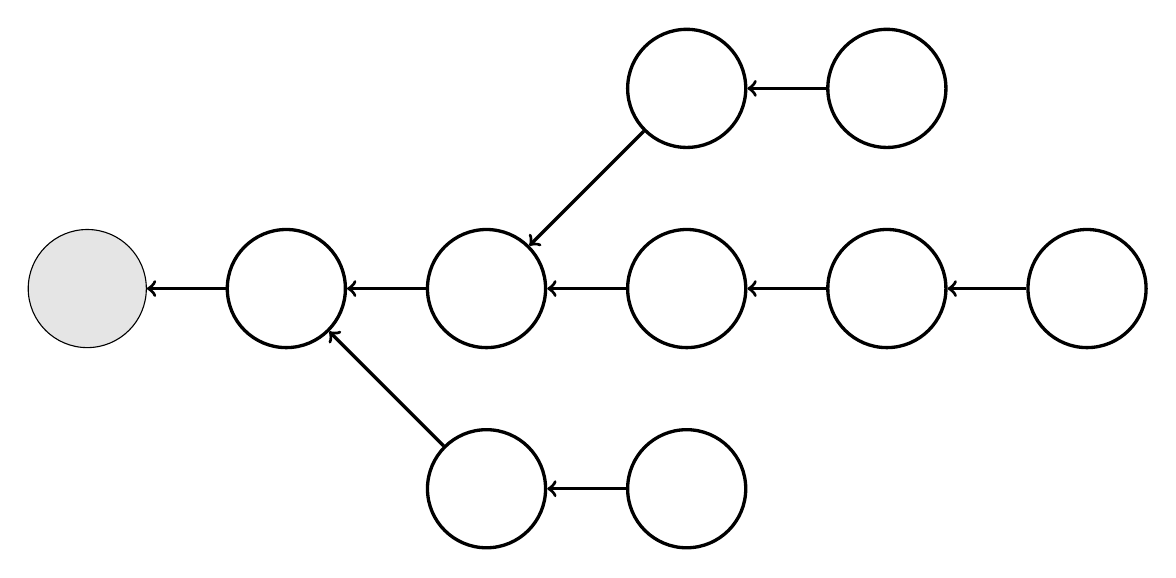
\begin{tikzpicture}[
				block/.style={circle, draw=black!100, very thick, minimum size=1.5cm},
				invis/.style={circle, draw=black!100, fill=black!10, minimum size=1.5cm}
			]
			\node[invis] (genesisblock) {};
			\node[block] (block1) [right=of genesisblock] {};
			\node[block] (block2) [right=of block1] {};
			\node[block] (block3) [right=of block2] {};
			\node[block] (block4) [right=of block3] {};
			\node[block] (block5) [right=of block4] {};
			\node[block] (sub1) [below=of block2] {};
			\node[block] (sub2) [below=of block3] {};
			\node[block] (sub3) [above=of block3] {};
			\node[block] (sub4) [above=of block4] {};
			\begin{scope}[very thick, -stealth]
			\draw[<-] (genesisblock.east) -- (block1.west);
			\draw[<-] (block1.east) -- (block2.west);
			\draw[<-] (block2.east) -- (block3.west);
			\draw[<-] (block3.east) -- (block4.west);
			\draw[<-] (block4.east) -- (block5.west);
			\draw[<-] (sub3.east) -- (sub4.west);
			\draw[<-] (block1.south east) -- (sub1.north west);
			\draw[<-] (sub1.east) -- (sub2.west);
			\draw[<-] (block2.north east) -- (sub3.south west); 
			\end{scope}
			\end{tikzpicture}
			\end{center}
		\caption{A typical blockchain structure}
		\label{fig:mainblockchain}
	\end{figure}
	The blockchain, as a cryptographically secure chain of blocks, was first conceptualised by Stuart Haber and W. Scott Stornetta in 1990 \parencite{10.1007/3-540-38424-3_32}.
	However, the most significant uses of the technology did not come until the creation of Git \parencite{Git} in 2005, and the invention of Bitcoin \parencite{Bitcoin} in 2008.
	Bitcoin uses the Proof of Work consensus algorithm to create a decentralised, trust-less, peer to peer network which is used to make transactions between virtual wallets.

	\section{Blockchain Today}
	At the time of writing, cryptocurrencies are generating both a huge amount of excitement and cynicism in popular media. 
	Aside from Bitcoin, cryptocurrencies like Ethereum \parencite{Ethereum} have introduced the concept of Smart Contracts which allow the execution of code on the blockchain.
	Whilst it is possible to think of applications for blockchain technology in almost every sector, the development of applications outside the scope of cryptocurrencies has been limited. 
	If one considers the example of OCaml, there are currently no libraries which allow a user to easily get started with building blockchain applications, and this is what Logan aims to change. \\

	\section{Work Completed}
	I have created Logan, a library that allows developers to create blockchain applications with the ease of importing a library.
	Logan was designed to exist outside the realm of cryptocurrencies and therefore assumes that all participants are trustworthy.
	Consensus is achieved by using a simple leader-based mechanism where the leader periodically pulls updates from participants and adds them to a central blockchain.
	This blockchain can viewed by all participants, with the guarantee of strict consistency.
	The system is also capable of running passive replication so that in the case of leader failure, the state of the leader at the point of failure can be manually recovered.
	To use Logan, all that a developer needs to specify is the location of the leader, participants and replicas, and to specify, if necessary, how the leader should perform validation.\\
	
	I have evaluated Logan's performance by observing how the transaction throughput that the system achieves varies with applied throughput, and by measuring how the latencies change as the blockchain size increases.
	My results showed that Logan is capable of dealing with throughputs and latencies which are much better than those achieved by Bitcoin.
	I have also shown that for a network with remote participants, the latency of adding transactions increases linearly with blockchain size. 
	This is undesirable as it means performance will degrade for long blockchains, however, I have been able to attribute this to the implementation of Git that Irmin/Ezirmin uses to pull updates over the network. 
	I have also shown that pure Git achieves a much better efficiency and that a better OCaml implementation of this protocol would allow Logan to achieve constant transaction latencies with blockchain size.
	Finally, I have shown that participant and replica nodes can be added to a Logan network with only a modest increase in transaction latencies.

	\chapter{Preparation}
	Before starting work on the project code, I completed a lot of preparation in order to aid the development process.
	I spent some time learning to use OCaml and familiarising myself with its features.
	This was important because it allowed me to write idiomatic code which was not only powerful, but could also provide an intuitive API for other developers to use.
	I also spent some time investigating Lwt which is an OCaml library that allows multi-threading through monadic `promises'.
	Setting up a good development environment allowed me to run automated builds and, therefore, catch any errors in the code early.
	This was particularly useful during the evaluation as it involved installing the project on many remote machines.
	Being able to catch issues like dependency resolution or out-of-date build commands made the evaluation process much easier.
	Lastly, I spent some time developing a requirements analysis for the final product. 
	This analysis helped drive the design and development of Logan as well as providing a baseline that was useful when evaluating its performance.

	\section{Starting Point}
	The project built upon functionality provided by Irmin \parencite{Irmin} which is a distributed data store system. Irmin is fast, durable and has all the necessary capabilities required to build a blockchain.
	The project also made use of Ezirmin \parencite{Ezirmin} which provides a simplified API to Irmin, and defines a log data structure which was used to build the blockchain and mempool structures for this project. 

	\section{Using OCaml}
	At the start of the project I had never used OCaml, so in the first few weeks of my project I spent time studying the book Real World OCaml \parencite{RealWorldOCaml} which proved a great introduction to many of OCaml's features.  
	In this section I will give a brief overview of some of OCaml's language features which are used in Logan's technical specification.
	I will then give a description of the development environment I set up during the course of the project.
	Finally I will give a description of the Lwt library for threading as it is extensively used in Logan's codebase and specification.

	\subsubsection*{Options}
	The first of OCaml's language features that I will is the \texttt{Option}.
	An \texttt{Option} is a built in data type that provides a powerful way of using OCaml's pattern matching.
	By using the \texttt{Some(\ldots)} and \texttt{None} constructors, one can create something of the type \texttt{'a option}. 
	This is comparable to the \texttt{null} type in languages such as Java, however as it is part of the type system, it forces the programmer to handle any cases where \texttt{null} could be returned. 

	\subsubsection*{Modules and Functors}
	Modules provide a way of grouping together related code in OCaml.
	They can be thought of as similar to traditional namespaces, although there are few key differences.
	OCaml also lets you define module type signatures which modules have to conform to.\\
	\begin{lstlisting}[caption={OCaml Modules and Functors},label={lst:modfun}]
module type Math = sig
  type t
  val add: t -> t -> t
  val subtract: t -> t -> t
end

module IntegerMath : Math with type t = int = struct
  type t = int
  let add int1 int2 = int1 + int2
  let subtract int1 int2 = int1 - int2
end
	\end{lstlisting}
	\noindent Listing \ref{lst:modfun} is a simple example that defines a module signature \texttt{Math} for adding and subtracting a custom type.
	The module \texttt{IntegerMath} is a module which adheres to this signature. 
	The syntax \texttt{with type t = int} lets the compiler know that the type t is externally visible.\\

	Modules are really useful for allowing the effective division of code into isolated units, but on their own, they are slightly inflexible. 
	For instance a developer might want to abstract some lower level details of code used by a module.
	In this case, she would have to create a whole new module for each possible implementation of this abstraction.
	Functors make this process much easier by allowing modules to be created from other modules. 
	This means that any lower level details can be passed into a module through the use of a functor.
	An example drawn from Ezirmin is a \texttt{Log}. 
	This is datastore that uses either an in-memory or on-disk format for storing data as shown in Listing \ref{lst:logmod}.\\
	\begin{lstlisting}[caption={Ezirmin Log Module},label={lst:logmod},float,floatplacement=H]
module Log(AO : Irmin.AO_MAKER)(V: Tc.S0) = struct
  ...
end
	\end{lstlisting}
	\noindent The parameter \texttt{AO} is a module used for creating append only stores, and the parameter module \texttt{V} defines a data type.
	Both of these modules can be used within the struct, which allows a flexible backend implementation.
	The result of this is a functor, \texttt{Log}, which can be used to create a Log module with either an in-memory or on-disk backend.

	\subsubsection*{Development Environment}
	When developing a large scale system with OCaml, there are a couple of build systems available to use. 
	jbuilder \parencite{jbuilder} is one of these systems which is becoming increasingly popular and is used daily by hundreds of developers.
	jbuilder allows the developer to specify arbitrary directory structures containing executables, libraries and more.
	I set up my jbuilder project to compile Logan, which includes the interface for running both leader and participant nodes. 
	I also defined multiple executables for running both the leader and participants in example and test cases. 
	I used GNU Make \parencite{GNUMake} to invoke jbuilder which allowed me to easily build and run any executables from the root of the directory.\\
	
	In order to ensure that the project would always build, I set up a continuous integration workflow using Travis-CI. 
	This ensured that whenever I pushed any updates to my GitHub repository, Travis would attempt to build the system and would notify me whenever there were any errors during the build.
	This was particularly useful during the evaluation stage when I was installing my project on multiple remote machines for testing.
	Over the development period, Travis flagged issues such as dependency resolution failures or out of date build scripts, and I was able to fix these at the point when they first occurred, rather than weeks later when they would have caused many issues during remote installation.

	\subsubsection*{Lwt}
	Lwt \parencite{Lwt} is a library which I spent some time familiarising myself. 
	Lwt provides a way of interacting with threads in OCaml, although in Lwt they are known as `Promises'.\\
	\begin{lstlisting}[caption={Lwt Promises},label={lst:lwt}]
val Lwt.return : 'a -> 'a Lwt.t 
val Lwt_main.run : 'a Lwt.t -> 'a
val Lwt.bind : 'a Lwt.t -> ('a -> 'b Lwt.t) -> 'b Lwt.t
	\end{lstlisting}
	\noindent Listing \ref{lst:lwt} shows the basic functions for creating, running and combining threads.
	The type \texttt{'a Lwt.t} refers to a thread which will eventually terminate with a value of type \texttt{'a}, and follows the well established Monad design pattern.
	\texttt{Lwt.return} is a function that takes a value and will create a promise that immediately returns with this value.
	This is useful when inserting static or precomputed variables into Lwt pipelines.
	\texttt{Lwt\_main.run} is the dual of \texttt{Lwt.return} and will run a Lwt promise until completion and then return its value.
	This is useful when retrieving values from an Lwt pipeline.
	Finally, \texttt{Lwt.bind} (or the infix notation \texttt{>>=}) will pass the result of a Lwt promise to a function returning another Lwt promise.
	This is useful for chaining together Lwt promises in a pipeline.

	\section{Requirements Analysis} \label{Requirements Analysis}
	During the preparation stage of my project, I spent some time analysing the requirements that would be suitable for Logan. 
	This proved a good way of guiding the progress of the project and making sure that the final result had satisfactory performance. 
	Here, I will set out the criteria that I decided upon before starting development on the project.

	\subsection{Data Structure}
	It is required that any node in a Logan network should be able to add items to and view items in the blockchain. 
	The data in the blockchain will be referred to as either \textit{blocks} or \textit{transactions}\footnote{The terms `block' and `transaction' will be used interchangeably in this report, however in general, systems will have blocks that contain multiple transactions. In Logan, this feature can be reproduced if the developer specifies a block data type that contains multiple transactions.}. 
	From a participant, it should be possible to add transactions of arbitrary type. 
	It should also be possible to view an ordered list of all transactions which currently exist in the blockchain.
	The latency of adding transactions should not increase as the size of the blockchain increases because it is important the library will cope well for systems with extremely long blockchains.\\

	\begin{lstlisting}[caption={Blockchain Specification},label={lst:blockspec},float,floatplacement=H]
module type I_LogStringCoder = sig
  type t
  val encode_string: t -> string
  val decode_string: string -> t option
end

module type I_Validator = sig 
  type t 
  val init: t list -> unit Lwt.t 
  val filter: t list -> t list Lwt.t
end

module type I_Config = sig
  type t
  module LogCoder: I_LogStringCoder with type t = t
  module Validator: I_Validator with type t = t
  val remotes: string list
end

module type I_Blockchain = sig
  type t
  val add_transaction_to_blockchain: t -> [> `Error | `Ok] Lwt.t
  val get_all_transactions: unit -> [> `Error | `Ok of t list] Lwt.t
  val get_transactions: int -> [> `Error | `Ok of t list] Lwt.t
end

module Make(Config: I_Config): I_Blockchain with type t = Config.t = struct 
  ...
end
	\end{lstlisting}
	In Logan, a blockchain module is used to add and view transactions in the blockchain.
	This blockchain module is created by a functor called \texttt{Make}.
	This functor accepts an \texttt{I\_Config} module which defines how transactions are to be validated, and configuration details including the list of participating nodes and a module defining how data can be serialised and deserialised.
	Listing \ref{lst:blockspec} is the initial technical specification that I used to define Logan, and the purpose of each component is as follows: 
	\begin{itemize}
		\item \texttt{I\_Config} contains information which is required to run the blockchain, including \texttt{remotes} which is a list of other participating nodes.
		\item \texttt{I\_LogStringCoder} is a module that allows the user to specify arbitrary types to be stored on the blockchain, so long as they can be encoded to (and decoded from) a string.
		\item \texttt{I\_Validator} is an interface which is defined by the library user. 
		Validation is performed by initialising a \texttt{Validator} module with the transactions already committed to the blockchain.
		From then on, \texttt{Validator.filter} will take a list of requested transactions and will return a subset of them which are the valid transactions.
		The \texttt{Validator} can then assume that these transactions have been committed for future calls to \texttt{filter}.
		\item \texttt{Make} is a functor which accepts a configuration module and will return a blockchain module.
		\item \texttt{add\_transaction\_to\_blockchain} adds a user defined type to the blockchain and then returns a polymorphic variant type containing information about whether the operation was successful. 
		This will return an error in the case that the transaction is not validated.
	\end{itemize} 
	This specification differs slightly from the final specification for Logan because it does not take into account the difference between leader and participant nodes.
	The specification was deliberately designed \textit{without} focus on consensus.
	It specifies solely the user facing components of the system because the way the system achieves consensus should be transparent to the developer.
	The final interface differs from this specification slightly to take into account the different roles of leaders and participants, however, it fundamentally provides exactly the same functionality.

	\subsection{Consensus}\label{Consensus Requirements}
	Ensuring that Logan maintains consensus was a very crucial part of this project. 
	The actual design and development of the consensus algorithm was completed throughout the duration of the project and involved a lot of research into other consensus mechanisms.
	However, during the requirements analysis phase of the project I set out some goals for the final implementation.
	These goals were laid out in order to help drive the design and development of the consensus mechanism. 
	I decided on the following success criteria which I have given names that are used in the evaluation section:
	\begin{itemize}
		\setlength{\itemindent}{2em}
		\item[\textbf{SC\_1}]The consensus mechanism must guarantee strict consistency in the blockchain state. 
		Although strict consistency could add large overhead costs, it is necessary for some applications and so is an important part of the final project.
		\item[\textbf{SC\_2}] As a baseline, Bitcoin achieves a maximum throughput of roughly 10 transactions per second (tps) \parencite{ScalingBitcoin}.
		Logan should be able to achieve comparable throughputs.
		\item[\textbf{SC\_3}] Again as a baseline, transaction latency achieved by Bitcoin is more than 10 minutes \parencite{ScalingBitcoin}.
		This is widely regarded as poor performance so Logan should be able to achieve better latencies of under a minute.
		\item[\textbf{SC\_4}] The latency of adding a block should be constant in the size of the blockchain.
		\item[\textbf{SC\_5}] The consensus mechanism must be scalable. 
		Within the scope of this project, it should be possible for the blockchain to be shared by 3 nodes in a network. 
		Latencies will inevitably grow with the number of nodes in the network, as is the case in most distributed systems.
		Logan's performance should demonstrate only modest decreases in performance for increases in nodes in a network.
	\end{itemize}

	\chapter{Implementation} \label{Implementation}
	Over the course of this project I have built Logan, a blockchain library which can perform custom transaction validation.
	Logan uses a leader-based consensus protocol inspired by Raft \parencite{Raft} and also uses the concept of a `transaction waiting room', or \textit{mempool}, which is used by Bitcoin.
	Section \ref{sec:sysarch} gives a general overview of Logan's system architecture.
	Section \ref{sec:datastructure} describes the blockchain data structure that I have used, and justifies why it can be considered a blockchain.
	I will also describe two bugs that I encountered in these codebases and the fixes that I implemented for each.
	Finally, Section \ref{sec:consensus} gives a description of Logan's consensus mechanism. 
	I will first present a na\"{i}ve approach to consensus and explain why this is flawed and may cause participants to temporarily view alternate orderings of blocks in the blockchain.
	I will then present an improved mechanism, which Logan uses, that guarantees correct ordering of requested transactions.
	Lastly, I will explain how Logan can achieve passive replication that allows the latest leader state to be recovered after a leader failure.
	This is a simple approach to fault tolerance but will show how a more complex approach could be incorporated.

	\section{System Architecture}\label{sec:sysarch}
	Logan's goal is to allow multiple nodes in a distributed system to share a blockchain data structure.
	Nodes in this system should be able to add transactions to the blockchain and read the entire history of previous transactions.
	I shall refer to blocks in the blockchain as \textit{transactions} as if they contain only a single transaction, however they can easily be made to contain many transactions because the datatype of transactions is arbitrary and specified by the developer.
	Logan aims to achieve consensus by using a centralised leader-based approach where a leader can accept transactions from participants and commit them to the blockchain for everyone to see.
	Participants view the blockchain by retrieving the latest copy over the network from the leader.
	Participants request for transactions to be committed by writing to their local mempool. 
	The leader periodically polls the participant mempools over the network to find new transactions to add to the blockchain.
	When the leader finds new transactions, it will use the validation module to filter all the valid transactions and add them to the blockchain.
	If necessary, the leader will first push these changes to the specified replicas.
	It is also possible for a participant node to exist on the same physical machine as the leader, in which case the leader sources updates directly from the mempool, rather than over a network connection. 
	Figure \ref{fig:sysarch} shows how the architecture for this system is organised.\\	

	\begin{figure}
		\centering
		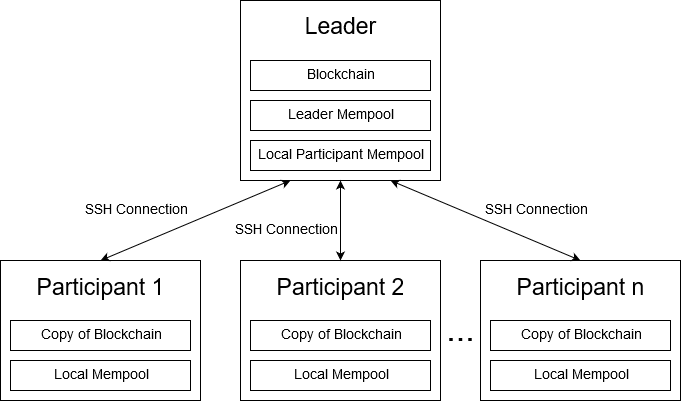
\includegraphics[width=16cm]{figs/System_Architecture.png}
		\caption{Logan system architecture overview}
		\label{fig:sysarch}
	\end{figure}

	\section{The Blockchain Data Structure}\label{sec:datastructure}
	Irmin  \parencite{Irmin} is a library for OCaml providing datastore functionality using a Git backend.
	Ezirmin is a wrapper around Irmin that provides a simple log data structure which I have used as a blockchain.
	In order to justify that this data structure can be considered a blockchain, I took some time to investigate its semantic properties. 
	Whilst there is no universally agreed-upon definition of a blockchain, I have used the following two criteria to define the blockchain:
	\begin{enumerate}
		\setlength{\itemindent}{2em}
			\item[\textbf{DS\_1}] Data is stored in `blocks'.
			\item[\textbf{DS\_2}] Blocks are ordered in a tree-like structure where each block contains the hash its parent block.
	\end{enumerate}
	This definition deliberately makes no mention of consensus, and exists purely to justify the validity of the blockchain data structure.
	\subsection{Irmin}
	Irmin exposes three main structures as shown in Figure \ref{fig:IrminBlockStore}: The Block Store, the Tag Store and the Irmin Store.
	\begin{figure}
		\begin{center}
		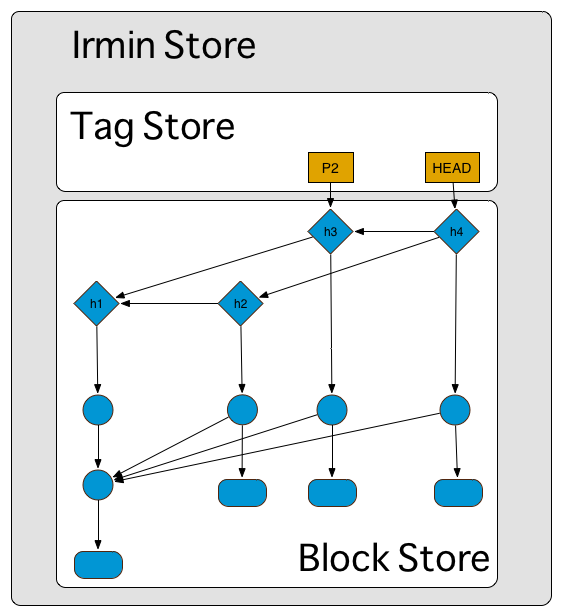
\includegraphics[width=13cm]{figs/irmin-stores.png}
		\caption{Architecture of an Irmin store}
		\label{fig:IrminBlockStore}
		\end{center}
	\end{figure}
	For the reader familiar with Git, these can intuitively be thought of as objects/commits, branches and repositories respectively.
	\subsubsection*{The Block Store}
	The Irmin Block Store is a heap of immutable blocks. 
	Rather than being addressed by a physical address, these blocks are addressed by the hash of their content.
	Because the Block Store is content-addressable, once blocks are added, their content can never be updated.
	Instead, updates to Irmin data structures are always made by adding new blocks to the store.
	These new blocks can link to old blocks or replace them entirely depending on the data structure.
	\subsubsection*{The Tag Store}
	Any mutability in Irmin data structures derive from \textit{tags}.
	Tags provide a way of indexing into any block in the Block Store.
	This concept is similar to that of branches or references in Git, which provide a way of indexing into a particular commit in the Git history.
	Because blocks are immutable, any changes to an Irmin data structure can only be visible if a tag is updated to point to a different block. 
	In this report, I will refer to the HEAD tag, which indexes into the latest recognised log item.
	When Irmin merges data structures, it creates new blocks and updates the relevant tags to point to these, however, the old blocks remain in the block store.
	\subsubsection*{Irmin Stores}
	An Irmin Store is simply the combination of a Block Store and a Tag Store.
	Considering the criteria set out earlier for a data structure to be considered a blockchain, Irmin Stores satisfy \textbf{DS\_1}.
	Indeed, they also come close to satisfying \textbf{DS\_2}, as all blocks are indexed by the hash of their content. 
	However, this is not quite enough, as blocks are not required to contain hashes of parents in a chain.
	In order to satisfy this criteria, I looked to Ezirmin which provides a log data structure.

	\subsection{Ezirmin}
	Ezirmin is a library that provides a simplified interface to the Irmin library. 
	Importantly, it has a built in log data structure which uses Irmin's append-only store, saved on disk in the Git format. \\

	\begin{lstlisting}[caption={Ezirmin Log},label={lst:ezirminlog}]
module type FS_Log = sig
  type elt 
  type cursor 
  val append : ?message:string -> branch -> path:string list -> elt -> unit Lwt.t
  val get_cursor : branch -> path:string list -> cursor option Lwt.t
  val read : cursor -> num_items:int -> (elt list * cursor option) Lwt.t
  val read_all : branch -> path:string list -> elt list Lwt.t
  ...
end
	\end{lstlisting}

	Listing \ref{lst:ezirminlog} gives some of the interface for an Ezirmin log which uses a file system backend.
	The log provides the functions \texttt{append} and \texttt{read} which allow for items to be appended to and read from a log.
	Additionally, the log uses a \texttt{cursor} type which is simply an abstraction for Irmin tags.
	A cursor to the latest item in a branch can be created with the function \texttt{get\_cursor}.

	\subsubsection*{Ezirmin Log as a Blockchain}
	Logan uses an Ezirmin Log as an implementation of a blockchain, and to verify that this is a valid data structure to use, I investigated the implementation of Ezirmin Logs.
	Ezirmin Logs use Irmin blocks to store log entries, and therefore satisfy \textbf{DS\_1}. 
	To verify that they also satisfy \textbf{DS\_2} I looked at the implementation of log items.\\

	\begin{lstlisting}[caption={Ezirmin Log Item},label={lst:a_label}]
type log_item =
{ time    : Time.t;
  message : V.t;
  prev    : K.t option}
	\end{lstlisting}

	Listing \ref{lst:a_label} is taken from the Ezirmin Log implementation and shows how each log item has a \texttt{prev} value which is a key pointing to its parent log item. 
	Because keys in Irmin are also hashes, this means that an Ezirmin log forms an ordered chain of blocks, each containing the hash of its parent. 
	Therefore, this satisfies \textbf{DS\_2}.

	\subsubsection*{Merging Ezirmin Logs}
	Ezirmin logs usually store each log item in a \texttt{Value} block.
	This is not always the case as merging updates from other logs may cause new \texttt{Merge} blocks to be created that collate and order the log entries which do not exist in both logs.
	These entries are ordered by their timestamps and this means that after a merge, items may appear to have been inserted into the log history.
	This behaviour is demonstrated in Figure \ref{fig:ezirminmerges}.
	For a blockchain, this would mean that multiple participants may observe different orderings depending on whether they view the blockchain before or after a merge.
	This is not desirable behaviour for a blockchain, so I have ensured that the blockchain data structure maintained by Logan is never merged with other structures, only appended to. 
	Consequently, each blockchain transaction will exist in its own \texttt{Value} block and will never removed or reordered in the blockchain.
	Therefore, an Ezirmin Log satisfies both of my conditions to be considered a blockchain.\\

	Aside from using an Ezirmin Log as the blockchain data structure for this project, I have also used a \textit{mempool} log to retrieve updates/transactions from remote mempools. 
	This retrieval process uses the \texttt{Ezirmin.Repo.Sync} module to merge new log items into the leader's mempool.
	Under the hood, this module uses the OCaml Git to pull updates over the network.\\

	\begin{figure}
		\centering
		\begin{subfigure}[t]{0.40\textwidth}
			\centering
			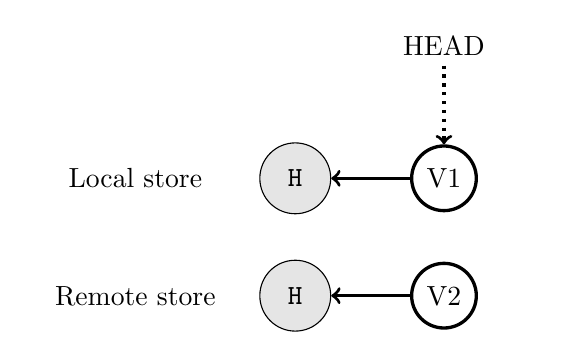
\begin{tikzpicture}[
				block/.style={circle, draw=black!100, very thick, minimum size=7mm},
				invis/.style={circle, draw=black!100, fill=black!10, minimum size=9mm},
				label/.style={rectangle, text width=2.5cm, align=center}
			]
			\node[label] (local) {Local store};
			\node[label] (remote) [below=of local] {Remote store};
			\node[invis] (gentop) [right=2mm of local]{\texttt{H}};
			\node[block] (history1) [right=of gentop] {V1};
			\node[label] (head) [above=of history1] {HEAD};
			\node[invis] (genbottom) [right=2mm of remote] {\texttt{H}};
			\node[block] (history2) [right=of genbottom] {V2};
			\begin{scope}[very thick, -stealth]
			\draw[->, dotted] (head.south) -- (history1.north);
			\draw[<-] (gentop.east) -- (history1.west);
			\draw[<-] (genbottom.east) -- (history2.west);
			\end{scope}
			\end{tikzpicture}
		\caption{Two Ezirmin logs diverging from a shared history, \texttt{H}.}
		\end{subfigure}
		\hspace{0.08\textwidth}
		\begin{subfigure}[t]{0.5\textwidth}
			\centering
			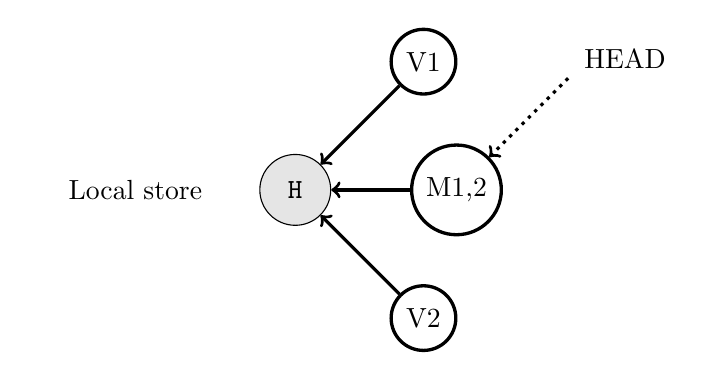
\begin{tikzpicture}[
				block/.style={circle, draw=black!100, very thick, minimum size=7mm},
				invis/.style={circle, draw=black!100, fill=black!10, minimum size=9mm},
				label/.style={rectangle, text width=2.5cm, align=center},
				labelhead/.style={rectangle, text width=1.2cm, align=center}
			]
			\node[label] (local) {Local store};
			\node[invis] (gentop)[right=2mm of local] {\texttt{H}};
			\node[block] (history1) [above right=of gentop] {V1};
			\node[block] (history2) [below right=of gentop] {V2};
			\node[block] (merge) [right=of gentop] {M1,2};
			\node[labelhead] (head) [above right=of merge] {HEAD};
			\begin{scope}[very thick, -stealth]
			\draw[->, dotted] (head.south west) -- (merge.north east);
			\draw[<-] (gentop.north east) -- (history1.south west);
			\draw[<-] (gentop.south east) -- (history2.north west);
			\draw[<-] (gentop.east) -- (merge.west);
			\end{scope}
			\end{tikzpicture}
			\caption{After the local log has merged changes from the remote log, the HEAD tag now point to a merge item, \texttt{M1,2}, which is generated by the custom merge function.}
		\end{subfigure}
		\caption{Merging Ezirmin logs}	
		\label{fig:ezirminmerges}
	\end{figure}

	\subsubsection*{Ezirmin Bugs}
	Whilst Ezirmin provides a set of very desirable semantic properties, it is not a widely used library. 
	Consequently, during the course of the project, I encountered bugs in the Ezirmin codebase which I had to debug and fix.
	In this section I shall outline the two bugs that I encountered and the changes I made to the Ezirmin codebase to fix them.\\
	
	The first bug occurs when updates are merged into a log over a network.\footnote{The issue on GitHub can be found at \href{https://github.com/kayceesrk/ezirmin/pull/7}{https://github.com/kayceesrk/ezirmin/pull/7}}
	Irmin uses Git as a backend and in order to merge updates over a network, the \texttt{git pull} command is used.
	In Git, objects are stored as blobs on the leaves of a tree and \texttt{git pull} works by retrieving all blobs at the leaf nodes of the tree for a given branch.
	However in Ezirmin, blobs can contain pointers to other blobs, and \texttt{git pull} will not know to retrieve these blobs too.
	This will cause an error when Ezirmin tries to read these objects which do not actually exist locally. 
	The solution that I implemented to this problem is to use an \textit{internal} branch which contains an Irmin Store that explicitly tracks every blob in the log.
	Items are added to this Irmin Store on the internal branch every time they are added to the log.
	This operation inserts these blobs into the Git tree such that if \texttt{git pull} is performed on the internal branch, all the blocks required by the master branch will be retrieved.\\

	The second bug that I encountered derived from the merge behaviour of Ezirmin logs when there are more than two remote machines merging updates from each others' log\footnote{The issue on GitHub can be found at \href{https://github.com/kayceesrk/ezirmin/pull/8}{https://github.com/kayceesrk/ezirmin/pull/8}}.
	The issue is that when a \texttt{Merge} block is created, it may contain log items which, on other machines, are stored as \texttt{Value} blocks or as different \texttt{Merge} blocks.
	The result is that these are seen as divergent histories and Ezirmin does not perform any checks to detect or remove duplicate log items that occur in different contexts.
	This behaviour resulted from complex sequences of merge operations and so was difficult to reproduce, but in the worst case caused the size of the blockchain to grow exponentially with the number of merge operations performed.
	In one case, a log with 40 unique log items grew to be greater than 120,000 log items in size due to duplicates.
	I implemented a fix by removing duplicate log items when a merge operation takes place. 
	Duplicates are found by comparing the log item timestamps, and whilst this does not guarantee their individuality, the timestamps have such significant precision to make this highly unlikely.

	\section{Achieving Consensus}\label{sec:consensus}
	Building consensus was by far the most important part of work completed for this project. 
	In order to guide the design of the consensus mechanism, I completed an extensive amount of research on existing algorithms.
	This section will briefly summarise this research and my conclusions about their suitability for Logan.
	I will then present the resulting design for consensus which is a leader based approach, where participants can commit transactions to a mempool.
	The leader polls these mempools for updates, which are validated and then committed to the blockchain.
	This blockchain can be read by all participants, and provides a definitive source of ordered, committed transactions.

	\subsection{Existing Consensus Algorithms} 
	\subsubsection*{Proof of Work} 
	Proof of Work (PoW) is a consensus mechanism, used by many cryptocurrencies to avoid the double spending problem \parencite{Bitcoin}. 
	This mechanism uses the concept of \textit{miners} which are nodes that are searching for a particular \texttt{nonce} value, which when added to the block, causes its hash to be preceded by a certain number of zeros.
	The structure of blocks in this scheme is demonstrated by Figure \ref{figs:pow}. 
	The nonce value of a block can only be found by a random brute force search.
	\begin{figure}
		\centering
		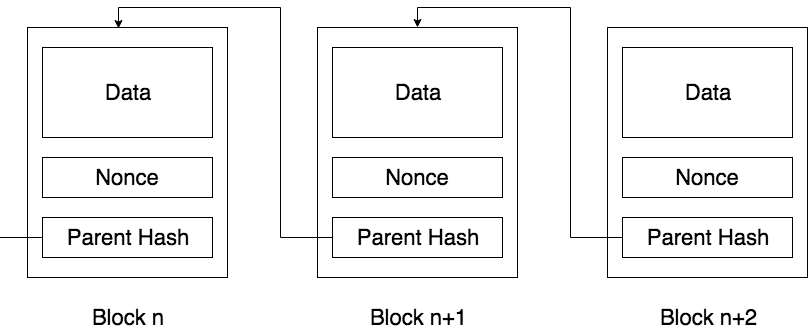
\includegraphics[width=13cm]{figs/PoW.png}
		\caption{Proof of Work block structure}
		\label{figs:pow}
	\end{figure}
	If the hash happens to be preceded by a certain number of zeros, this is considered a proof of computational work and the block is broadcast out to a network and added to every nodes copy of the blockchain.
	Because this process is completely random, it is impossible for an adversary with control over less than half the network to maintain a blockchain that is longer than the genuine blockchain for an indefinite amount of time.
	Participants can be more and more sure as the blockchain gets longer, that if a block is in the longest chain, then it is agreed upon by consensus. \\

	Importantly, this scheme assumes that no participant can be trusted 
	and this means that the consensus mechanism wastes a large amount of energy in the mining process \parencite{BitcoinEnergy}.
	It also assumes that miners can always be rewarded for mining and this may not always be true, so this scheme would not be suitable for some applications.
	
	\subsubsection*{Mempools}
	Mempools are an important part of the design of Bitcoin, and whilst they are not inherently linked to the Proof of Work consensus algorithm, they are worth investigating as they are used by Logan.
	When a Bitcoin transaction is made, it is first broadcast to all miners and written into their mempool. 
	These miners can choose to add these transactions to the next block they mine.
	This is significant, as it provides a `waiting room' for any transactions that have not yet been validated.\\

	In Logan, all participants have a mempool which can be read by the leader. 
	These mempools use the same Ezirmin log data structure that the blockchain uses and therefore, once a transaction is in the mempool, it is never removed. 
	This is not a requirement for the data structure and indeed a queue would be a more natural choice as it would allow transactions to be removed from the mempool after they had been read by the leader.
	Ezirmin provides a queue data structure but I have not used it in Logan because I anticipated encountering bugs similar to those I encountered with the log data structure, and a log is a sufficient data structure for a mempool.

	\subsubsection*{Proof of Stake}
	The Proof of Stake (PoS) algorithm \parencite{ProofofStake} is used by some cryptocurrencies and works by randomly allowing participants to create (or `forge') a single block.
	However, the probability that a participant is chosen to forge a block, is weighted by its stake, such that participants with higher stakes in the blockchain are more likely to be chosen to forge a block.
	With PoS, there is no need to waste lots of energy in the process of mining. 
	Using PoS also allows trust to be distributed according to an arbitrary heuristic which can be desirable property in some applications.\\

	Unfortunately, the notion of stake that is used by PoS may not always be available in the design of a general blockchain system. 
	It also, like PoW, assumes no trust in participating nodes and is therefore not suitable for use in Logan, which inherently assumes all nodes can be trusted.

	\subsubsection*{Paxos}
	Paxos is a family of consensus protocols which can be used to guarantee consistency in distributed systems. 
	It was first proposed in a paper by Leslie Lamport in 1998 \parencite{Paxos}, although the paper was first submitted in 1990.
	The main part of the algorithm is split into two sections, `propose' and `accept'.
	In the propose stage, a value is proposed by a node to all other nodes, and other nodes make a promise to accept.
	In the accept stage the value is accepted if a quorum of nodes made a promise to accept and then actually accept the value.\\

	Paxos has many issues including unspecified behaviour in certain situations, lack of guaranteed progress and overhead of implementation.
	I have not used it in this project but I have partially taken inspiration from the Roles used by Paxos in the design of my leader based protocol.

	\subsubsection*{Raft}
	Raft \parencite{Raft} is an algorithm that was designed to be equivalent and as efficient as Paxos, however, it also places a much greater emphasis on comprehensibility.
	It uses the notion of a \textit{strong leader}, which is an elected server that has total control over which log entries are accepted.
	If the leader does not send a heartbeat message within a certain timeout period, other nodes in the network will detect this and start an election for a new leader.\\
	
	Raft is an simple algorithm that is easy to understand, but it also guarantees the \textit{Log Matching Property} that if two logs contain a log entry with the same index and term, then that entry, and all preceding entries will be identical.
	The notion of a strong leader used in Logan is inspired by Raft.

	\subsection{Roles in a Logan's Approach}
	Logan uses a mempool and a simple leader-based algorithm that is inspired by the previously described consensus protocols.
	As I am assuming that all participants can be trusted, it is possible to use a leader based approach without introducing security issues such as the ones tackled by the Proof of Work mechanism. 
	Because I have implemented a centralised algorithm, Logan's specification differs slightly from the requirements analysis.
	This is accounted for by the differing functional requirements for a leader and for a participant, which are not considered in the requirements analysis.
	In this section I will describe the roles of different nodes in a Logan network, and I will present their new functional specification.
	
	\subsubsection*{Leaders}
	Logan uses the notion of a \textit{strong leader} similar to that used by the Raft protocol. 
	The leader is chosen statically in order to reduce the complexity of implementation, and it also has a statically defined list of remotes which specifies the location of all participants.
	In this approach the leader never actually requests transactions to be added to the blockchain, its role is simply to continuously read requests from the mempools of participants, validate them, and then add them to the blockchain.
	To add transactions from a leader's machine, a separate participant program must be run.
	The leader's blockchain can be read by any participant, and is treated as the empirical source of which transactions have been committed and in which order, with the guarantee that any ordering of blocks seen in the blockchain is final and will not change.
	This property is very similar to the Log Matching Property guaranteed by Raft, only with no notion of indexes or terms.\\

	\begin{lstlisting}[caption={Leader Specification},label={lst:leaderspec}]
module type I_LeaderConfig = sig
  type t
  module LogCoder: Participant.I_LogStringCoder with type t = t   
  module Validator: I_Validator with type t = t 
  val remotes: string list
  val replicas: string list
end

module type I_Leader = sig
  val init_leader: unit -> (unit -> unit Lwt.t) Lwt.t
end

module MakeLeader (Config: I_LeaderConfig) : I_Leader = struct
  ...
end
	\end{lstlisting}

	Listing \ref{lst:leaderspec} is the specification of the leader module, which differs slightly from the specification presented in the requirements analysis.
	In particular, \texttt{init\_leader} performs an initialisation step, and then returns a function which, when executed, will actually start the consensus process.

	\subsubsection*{Participants}
	Participants, in contrast to leaders, can request transactions to be added to the blockchain. 
	This is done by writing a transaction to a local mempool, which is then read by the leader in its next poll.\\

	\begin{lstlisting}[caption={Participant Specification},label={lst:partspec}]
module type I_LogStringCoder = sig
  type t
  val encode_string: t -> string
  val decode_string: string -> t option
end

module type I_ParticipantConfig = sig
  type t
  module LogCoder: I_LogStringCoder with type t = t
  val leader_uri: string option
end

module type I_Participant = sig
  type t
  val add_transaction_to_mempool: t -> [> `Could_Not_Pull_From_Remote | `Validation_Failure | `Ok] Lwt.t
  val get_transactions_from_blockchain: int -> [> `Error | `Ok of t list] Lwt.t
  val get_all_transactions_from_blockchain: unit -> [> `Error | `Ok of t list] Lwt.t
end

module Make(Config: I_ParticipantConfig): I_Participant with type t = Config.t = struct
  ...
end
	\end{lstlisting}

	Listing \ref{lst:partspec} is a specification that demonstrates the role of participants and the functionality they provide.
	It differs from Listing \ref{lst:blockspec} slightly in that it now contains the function \texttt{add\_transaction\_to\_mempool} rather than \texttt{add\_transaction\_to\_blockchain}.
	Aside from this, the specification is the same.

	\subsubsection*{Replicas}
	Replicas are nodes which contain the latest copy of the blockchain. 
	I shall explain later how fault tolerance can be introduced by ensuring that transactions only exist on the visible blockchain once they have been recognised by a quorum of replicas.
	Replicas are useful because the leader is a single point of failure, and if it fails, it is important to have another machine which can recover the state of the leader just before the point of failure.
	
	\subsection{Retrieving Updates from Mempools}
	A leader operates by pulling updates from participant mempools and then adding them to the blockchain.
	However, it is important that the leader does not miss transactions or commit transactions out of order.
	This is tricky because after pulling updates from many mempools the local copies will reflect each mempool at different moments in time.
	In this section, I will give the \textit{immediate commit approach} for retrieving and adding updates to the blockchain and I will show how this method is flawed. 
	This will then motivate the design of the \textit{delayed commit approach}, which Logan implements, that ensures all transactions are committed in order by holding them back for a full poll cycle.
	In both approaches, the leader will continuously poll mempools for updates and commit transactions that it believes to be valid. \\
	
	\subsubsection*{The Immediate Commit Approach}
	The first approach to retrieving updates from participants is to pull updates from all the participants into separate branches of the leader's mempool.
	The leader can see which updates have just been retrieved for each mempool by maintaining a \textit{latest known cursor} that points to the latest transaction seen by the leader, i.e. in its last poll.
	Figure \ref{fig:readmemudpates} shows how the \textit{latest cursor}, \texttt{LC}, which points to the latest item in the mempool, is used to retrieve updates.
	In this diagram the dotted nodes represent transactions that have been pulled in the latest poll.
	The leader can traverse back through the log from this cursor until it reaches the latest known cursor, \texttt{LKC}, and then it can return the newly found updates.
	\begin{figure}
		\centering
		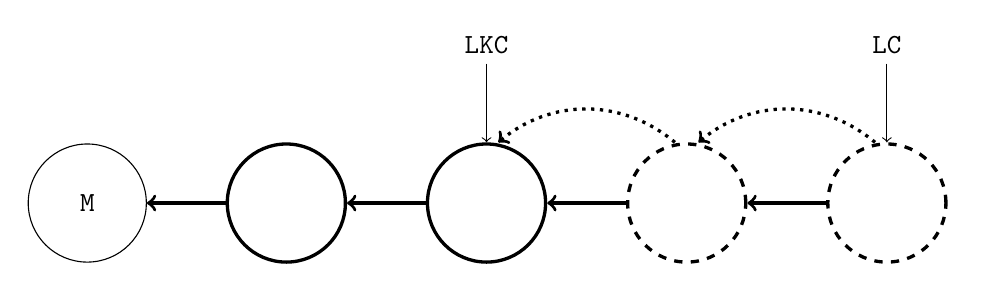
\begin{tikzpicture}[
			block/.style={circle, draw=black!100, very thick, minimum size=15mm},
			invis/.style={circle, draw=black!100, minimum size=15mm},
			label/.style={rectangle, text width=2cm, align=center}]                       
			\node[invis] (invis) {\texttt{M}};
			\node[block] (block1) [right=of invis] {};
			\node[block] (block2) [right=of block1] {};
			\node[label] (label1) [above=of block2] {\texttt{LKC}};
			\node[block] (block3) [right=of block2, dashed] {};
			\node[block] (block4) [right=of block3, dashed] {};
			\node[label] (label2) [above=of block4] {\texttt{LC}};
			\draw[->] (label2.south) -- (block4.north);
			\draw[->] (label1.south) -- (block2.north);
			\begin{scope}[very thick, -stealth]
				\draw[<-] (invis.east) -- (block1.west);
				\draw[<-] (block1.east) -- (block2.west);
				\draw[<-] (block2.east) -- (block3.west);
				\draw[<-] (block3.east) -- (block4.west);
				\path[dotted, ->] (block4.north)+(-1.5mm,0) edge  [bend right=40]  ([xshift=1.5mm]block3.north);
				\path[dotted, ->] (block3.north)+(-1.5mm,0) edge  [bend right=40]  ([xshift=1.5mm]block2.north);
			\end{scope}
		\end{tikzpicture}
		\caption{Retrieving updates from a single participant mempool}
		\label{fig:readmemudpates}
	\end{figure}
	Once the leader has retrieved all updates from the mempools of all participants, it can collate all these transactions into a single list ordered by their timestamp.
	This timestamp marks the time which transactions are added to the mempool on a participants machine.
	These transactions can be validated and added to the blockchain, and the \textit{latest known cursor} updated to the latest message in each of the mempool.
	Because these transactions are added as soon as they are recognised by the leader, this is known as the \textit{immediate commit approach}.\\

	However, this approach is fundamentally flawed and causes many updates to be seen out of order. 
	This is because the approach implicitly assumes that all updates from mempools can be retrieved instantaneously, and does not account for network delays.
	Figure \ref{fig:readremotepartudpatesbroke} demonstrates a typical situation where this occurs.
	The chains labelled \texttt{P} represent the mempools on the participants' machines and the middle chain represents the stream of updates as seen by the leader.
	In the figure, the leader pulls updates from the first worker before pulling updates from the second.
	After the pull from the first participant has completed and retrieved transaction 1, the first participant has added transaction 2 which has not been retrieved by the leader. 
	However, transaction 2 is timestamped before transaction 3 which is retrieved during the same poll cycle.
	In the immediate commit approach, transactions 1 and 3 will be added to the blockchain and transaction 2 will be retrieved and committed during the next poll.
	It will consequently come after transaction 3 even though it has an earlier timestamp, and this is not fair.
	This transaction also cannot be inserted into an earlier position of the blockchain because it would mean that different participants might observe the blockchain in diverging states.
	In other words it would break the equivalent property to Raft's log matching property which Logan claims to achieve.
	Because transaction 2 was missed during the first leader poll, I will refer to all such transactions as \textit{missed}.

	\begin{figure}
		\centering
		\begin{subfigure}[t]{0.40\textwidth}
			\centering
			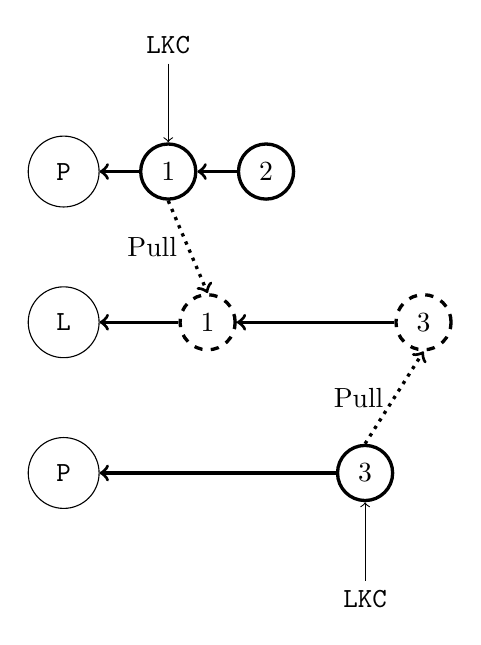
\begin{tikzpicture}[
				block/.style={circle, draw=black!100, very thick, minimum size=7mm},
				invis/.style={circle, draw=black!100, minimum size=9mm},
				label/.style={rectangle, text width=1.2cm, align=center}
			]
			\node[invis] (gentop) {\texttt{P}};
			\node[invis] (genmiddle) [below=of gentop] {\texttt{L}};
			\node[invis] (genbottom) [below=of genmiddle] {\texttt{P}};
			\node[block] (one) [right=5mm of gentop] {1};
			\node[block] (onemerged) [right=10mm of genmiddle, dashed] {1};
			\node[block] (two) [right=5mm of one] {2};
			\node[block] (three) [right=30mm of genbottom] {3};
			\node[block] (threemerged) [right=20mm of onemerged, dashed] {3};
			\node[label] (latestknownone) [above=of one] {\texttt{LKC}};
			\node[label] (latestknownthree) [below=of three] {\texttt{LKC}};
			\draw[->] (latestknownone.south) -- (one.north);
			\draw[->] (latestknownthree.north) -- (three.south);
			\begin{scope}[very thick, -stealth]
			\draw[<-] (gentop.east) -- (one.west);
			\draw[dotted, ->] (one.south) -- (onemerged.north) node[midway, left] {Pull};
			\draw[dotted, ->] (three.north) -- (threemerged.south) node[midway, left] {Pull};
			\draw[<-] (onemerged.east) -- (threemerged.west);
			\draw[<-] (one.east) -- (two.west);
			\draw[<-] (genmiddle.east) -- (onemerged.west);
			\draw[<-] (genbottom.east) -- (three.west);
			\end{scope}
			\end{tikzpicture}
		\caption{After first leader poll. Transactions 1 and 3 are recognised by the leader and added to the blockchain.}
		\end{subfigure}
		\hspace{0.09\textwidth}
		\begin{subfigure}[t]{0.40\textwidth}
			\centering
			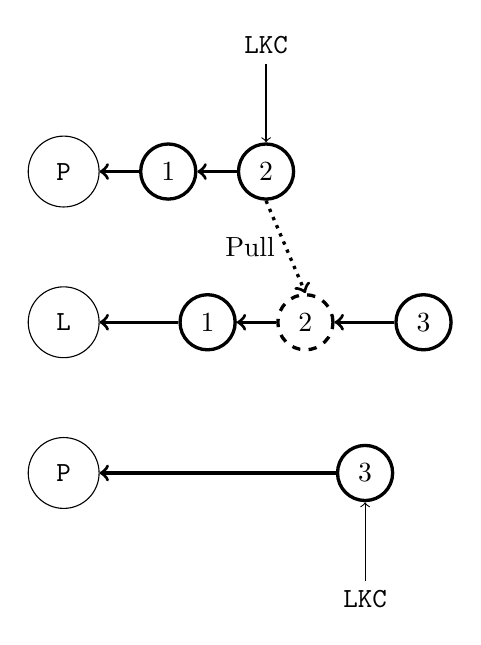
\begin{tikzpicture}[
				block/.style={circle, draw=black!100, very thick, minimum size=7mm},
				invis/.style={circle, draw=black!100, minimum size=9mm},
				label/.style={rectangle, text width=1.2cm, align=center}
			]
			\node[invis] (gentop) {\texttt{P}};
			\node[invis] (genmiddle) [below=of gentop] {\texttt{L}};
			\node[invis] (genbottom) [below=of genmiddle] {\texttt{P}};
			\node[block] (one) [right=5mm of gentop] {1};
			\node[block] (onemerged) [right=10mm of genmiddle] {1};
			\node[block] (two) [right=5mm of one] {2};
			\node[block] (twomerged) [right=5mm of onemerged, dashed] {2};
			\node[block] (three) [right=30mm of genbottom] {3};
			\node[block] (threemerged) [right=20mm of onemerged] {3};
			\node[label] (latestknowntwo) [above=of two] {\texttt{LKC}};
			\node[label] (latestknownthree) [below=of three] {\texttt{LKC}};
			\draw[->] (latestknowntwo.south) -- (two.north);
			\draw[->] (latestknownthree.north) -- (three.south);
			\begin{scope}[very thick, -stealth]
			\draw[<-] (gentop.east) -- (one.west);
			\draw[dotted, ->] (two.south) -- (twomerged.north) node[midway, left] {Pull};
			\draw[<-] (onemerged.east) -- (twomerged.west);
			\draw[<-] (twomerged.east) -- (threemerged.west);
			\draw[<-] (one.east) -- (two.west);
			\draw[<-] (genmiddle.east) -- (onemerged.west);
			\draw[<-] (genbottom.east) -- (three.west);
			\end{scope}
			\end{tikzpicture}
			\caption{After second leader poll. Transaction 2 is retrieved but should be ordered before transaction 3 in the blockchain.}
		\end{subfigure}
		\caption{Missing mempool updates with a na\"{i}ve consensus mechanism}	
		\label{fig:readremotepartudpatesbroke}
	\end{figure}
	\subsubsection*{The Delayed Commit Approach}
	In order to solve this problem, I first examined the nature of these \textit{missed} transactions and noted the following properties:
	\begin{enumerate}
		\item Any missed transactions must have been added whilst the leader was pulling updates. 
		If they had been added before the poll had begun, then they would have been retrieved in previous poll. 
		Therefore, \textit{missed} transactions must occur after the latest timestamped transaction from the previous poll. 
		\item Missed transactions must have been added at a point in time earlier than the latest update from the subsequent round of retrieved updates.
		If they occurred at a later point in time, then they would be correctly received in that subsequent leader poll.
	\end{enumerate}

	These properties naturally suggest a simple adjustment to the immediate commit approach, which only adds transactions to the blockchain if they have existed on the leader's machine for more than one poll cycle.
	For this reason, it is known as the \textit{delayed commit approach}.
	When a leader is first started and retrieves its first set of updates, it will add them to a \textit{retrieved} buffer.
	In the next poll cycle, the leader will transfer the retrieved buffer to a new \textit{to-be-committed} buffer.
	From now on, when the leader retrieves new updates from mempools it will do one of two things for each newly retrieved transaction:
	\begin{itemize}
		\item If a transaction has an earlier timestamp than the latest transaction in the to-be-committed buffer, the leader will insert it into the correct position in the to-be-committed buffer based on its timestamp.
		\item If a transaction has a later timestamp than the latest transaction in the to-be-committed buffer, the leader will add it to the retrieved buffer.
	\end{itemize}
	Then, all the leader has to do is validate the transactions in the to-be-committed buffer and add them to the blockchain.
	Figure \ref{fig:complexconsensusfix} demonstrates how this approach solves the problem presented in Figure \ref{fig:readremotepartudpatesbroke}.
	In Figure \ref{a}, transaction 2 has been missed whilst transactions 1 and 3 have been added to the retrieved buffer. 
	In Figure \ref{b}, transactions 1, 2 and 3 have all been inserted into the to-be-committed buffer and will be added to the blockchain.
	Transaction 4 has occurred after the latest item in the to-be-committed buffer, i.e. transaction 3, and is therefore added to the retrieved buffer instead. 
	So now that the previously described nature of missed transactions has been accounted for, it can be guaranteed that all transactions will be committed to the blockchain in the order that they were committed to their participants mempools.
	Neither the immediate commit nor the delayed commit approach takes participant failure into account and this could potentially stall progress of the leader. 
	However, this could be very easily accounted for with a timeout mechanism similar to the leader timeout used in Raft.\\

	\begin{figure}
		\centering
		\begin{subfigure}[t]{\textwidth}
			\centering
			\begin{tikzpicture}[
				block/.style={circle, draw=black!100, very thick, minimum size=7mm},
				invis/.style={circle, draw=black!100, minimum size=9mm},
				label/.style={rectangle, text width=1.2cm, align=center},
				buffer/.style={rectangle, align=center},
				bufferitem/.style={rectangle, draw=black!100, align=center},
				spacer/.style={rectangle, text=white}
			]
			\node[invis] (gentop) {\texttt{P}};
			\node[invis] (genmiddle) [below=of gentop] {\texttt{L}};
			\node[invis] (genbottom) [below=of genmiddle] {\texttt{P}};
			\node[block] (one) [right=5mm of gentop] {1};
			\node[block] (onemerged) [right=10mm of genmiddle, dashed] {1};
			\node[block] (two) [right=5mm of one] {2};
			\node[block] (three) [right=30mm of genbottom] {3};
			\node[block] (threemerged) [right=20mm of onemerged, dashed] {3};
			\node[label] (latestknownone) [above=of one] {\texttt{LKC}};
			\node[label] (latestknownthree) [below=of three] {\texttt{LKC}};
			\draw[->] (latestknownone.south) -- (one.north);
			\draw[->] (latestknownthree.north) -- (three.south);
			\node[buffer] (bufferlabel) [right=2cm of threemerged] {Retrieved Buffer:};
			\node[bufferitem] (item1) [right=1cm of bufferlabel] {1};
			\node[bufferitem] (item2) [right=0mm of item1] {3};
			\node[spacer] (space1) [below=5mm of item1] {.};
			\begin{scope}[very thick, -stealth]
			\draw[<-] (gentop.east) -- (one.west);
			\draw[dotted, ->] (one.south) -- (onemerged.north) node[midway, left] {Pull};
			\draw[dotted, ->] (three.north) -- (threemerged.south) node[midway, left] {Pull};
			\draw[<-] (onemerged.east) -- (threemerged.west);
			\draw[<-] (one.east) -- (two.west);
			\draw[<-] (genmiddle.east) -- (onemerged.west);
			\draw[<-] (genbottom.east) -- (three.west);
			\end{scope}
			\end{tikzpicture}
		\caption{After first poll}
		\label{a}
		\end{subfigure}
		\begin{subfigure}[t]{\textwidth}
			\centering
			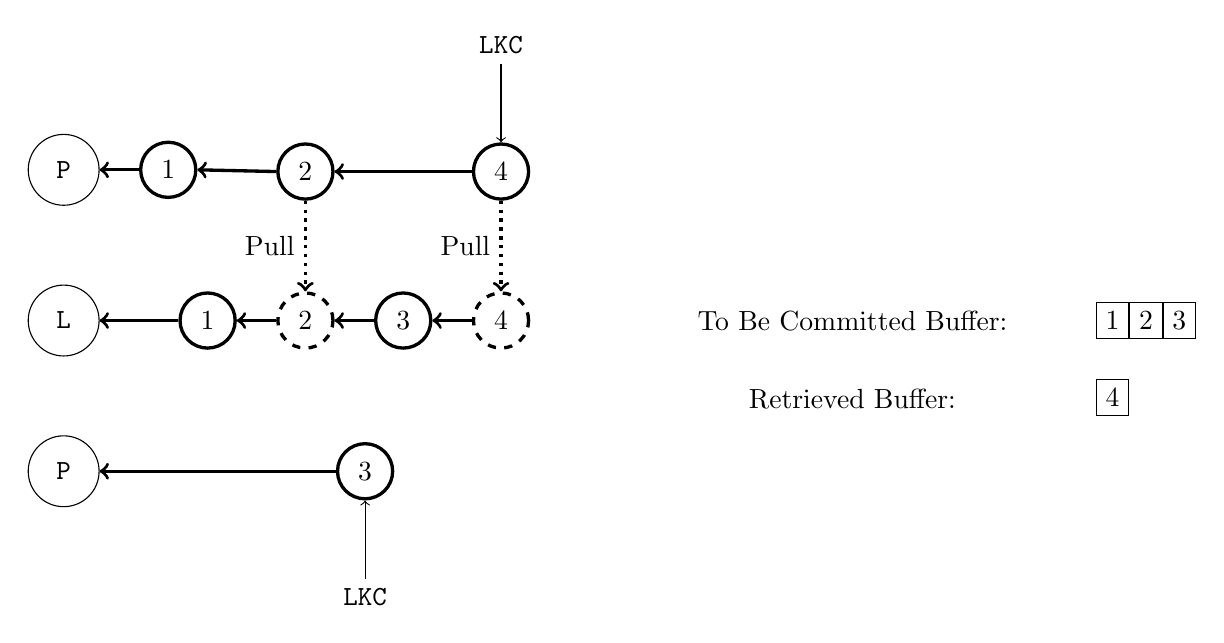
\begin{tikzpicture}[
				block/.style={circle, draw=black!100, very thick, minimum size=7mm},
				invis/.style={circle, draw=black!100, minimum size=9mm},
				label/.style={rectangle, text width=1.2cm, align=center},
				buffer/.style={rectangle},
				bufferitem/.style={rectangle, draw=black!100, align=center},
				spacer/.style={rectangle, text=white}
			]
			\node[invis] (gentop) {\texttt{P}};
			\node[spacer] (space) [above=1cm of gentop] {.};
			\node[invis] (genmiddle) [below=of gentop] {\texttt{L}};
			\node[invis] (genbottom) [below=of genmiddle] {\texttt{P}};
			\node[block] (one) [right=5mm of gentop] {1};
			\node[block] (onemerged) [right=10mm of genmiddle] {1};
			\node[block] (twomerged) [right=5mm of onemerged, dashed] {2};
			\node[block] (two) [above=1.15cm of twomerged] {2};
			\node[block] (three) [right=30mm of genbottom] {3};
			\node[block] (threemerged) [right=5mm of twomerged] {3};
			\node[block] (fourmerged) [right=5mm of threemerged, dashed] {4};
			\node[block] (four) [above=1.15cm of fourmerged] {4};
			\node[buffer] (txnslabel) [right=2cm of fourmerged] {To Be Committed Buffer:};
			\node[bufferitem] (item1) [right=1cm of txnslabel] {1};
			\node[bufferitem] (item2) [right=0mm of item1] {2};
			\node[bufferitem] (item3) [right=0mm of item2] {3};
			\node[label] (latestknownfour) [above=of four] {\texttt{LKC}};
			\node[label] (latestknownthree) [below=of three] {\texttt{LKC}};
			\draw[->] (latestknownfour.south) -- (four.north);
			\draw[->] (latestknownthree.north) -- (three.south);
			\node[buffer] (bufferlabel) [below=5mm of txnslabel] {Retrieved Buffer:};
			\node[bufferitem] (item1) [below=5mm of item1] {4};
			\node[spacer] (space1) [below=5mm of item1] {.};
			\begin{scope}[very thick, -stealth]
			\draw[<-] (gentop.east) -- (one.west);
			\draw[dotted, ->] (two.south) -- (twomerged.north) node[midway, left] {Pull};
			\draw[dotted, ->] (four.south) -- (fourmerged.north) node[midway, left] {Pull};
			\draw[<-] (onemerged.east) -- (twomerged.west);
			\draw[<-] (twomerged.east) -- (threemerged.west);
			\draw[<-] (one.east) -- (two.west);
			\draw[<-] (two.east) -- (four.west);
			\draw[<-] (genmiddle.east) -- (onemerged.west);
			\draw[<-] (genbottom.east) -- (three.west);
			\draw[<-] (threemerged.east) -- (fourmerged.west);
			\end{scope}
			\end{tikzpicture}
			\caption{After second leader poll}
			\label{b}
		\end{subfigure}
		\caption{Buffering updates in a complex consensus mechanism}	
		\label{fig:complexconsensusfix}
	\end{figure}

	\section{Tolerating Leader Failure}\label{sec:faulttol}
	Now that I have detailed Logan's data structures and the process through which it achieves consensus, the only aspect of the implementation left to consider is fault tolerance.
	Because Logan implements a leader-based consensus mechanism, this means that the leader is a single point of failure.
	In the event of a failure, different participants may have local copies of the blockchain at different times, or in other words, one participant's copy may contain some transactions which other participants' do not.
	Building full failure detection and recovery into Logan would be outside the scope of this Project. 
	Instead, in this section I will show the simple mechanism, that Logan uses, which allows manual recovery of the blockchain state in the case of a leader failure. 
	I will then explain how this leads to a bottleneck in the leader's execution before giving a more advanced mechanism which uses a daemon thread that removes the bottleneck from the leader's execution. 
	This solution was implemented, however because Git has very coarse grained locking, there were many race conditions and it was therefore not used in Logan's final implementation. 
	Nevertheless, I will describe this approach to demonstrate how Logan could operate if a protocol with finer grained locking was used. 
	This will justify that a more complex and automated approach to recovering from leader failure is possible, and will demonstrate a good starting point for implementing such a mechanism. \\

	To introduce fault tolerance, I have used \textit{replicas}. 
	Replicas, in computer science, are nodes which duplicate some part of another node's behaviour in order to allow recovery from failure. 
	They can be either \textit{active} if they fully duplicate the actions of another replica, or \textit{passive} if another machine completes some operation before transferring the result to that replica \parencite{Replication}.
	The replication I will demonstrate will be passive.\\

	In order to incorporate the notion of a replica, the process of adding commits to the blockchain needs to be altered slightly.
	Now, before a commit is made, it needs to be recognised by a quorum of replicas.
	Irmin's notion of branches exposes a perfect primitive for this application.
	In a poll, the leader can commit transactions to an uncommitted \textit{cache} branch before pushing this to all replicas.
	If a quorum of these push operations return successfully, then the leader can merge these transactions into the main blockchain branch to be viewed by all participants.
	If a failure were to occur at any point after this merge, it is now guaranteed that any transactions in the leader's blockchain will also exist on a quorum of replicas.
	This means that the system has access to sufficient information to reconstruct the contents of the blockchain before the failure.\\

	\begin{lstlisting}[caption={Naive Leader Loop},label={lst:leaderloop}]
let rec start_leader () = 
	retrieve_and_process_updates() >>= 
	commit_to_temporary_blockchain_branch >>=
	push_to_replica_quorum >>=
	merge_temp_branch_into_blockchain_master >>=
	start_leader
	\end{lstlisting}

	Listing \ref{lst:leaderloop} shows pseudocode for the leader's poll cycle, now incorporating replicas. 
	One of the major issues with this approach is that it introduces a bottleneck in the leader's execution which causes unnecessary delays.
	I propose a different approach that starts an asynchronous \textit{push-thread} which is in charge of pushing to replicas and merging the transactions which have been pushed.
	This thread is initially created by, but separate to, the \textit{main thread} which only commits items to a \textit{cache} branch.
	The push-thread operates by cloning the blockchain cache branch into a new \textit{push-cache} branch which it pushes to replicas.
	The difference between the cache and push-cache branches is that the cache branch will constantly be updated by the main thread as new transactions are retrieved from participants, whereas the push-cache branch will remain fixed containing a particular set of transactions whilst the push-thread pushes these to replicas. 
	When this push returns successfully, the push-cache thread will then merge this push-cache branch into the blockchain master branch, and loop. 
	\begin{figure}
		\centering
		\begin{subfigure}[t]{\textwidth}
		\centering
		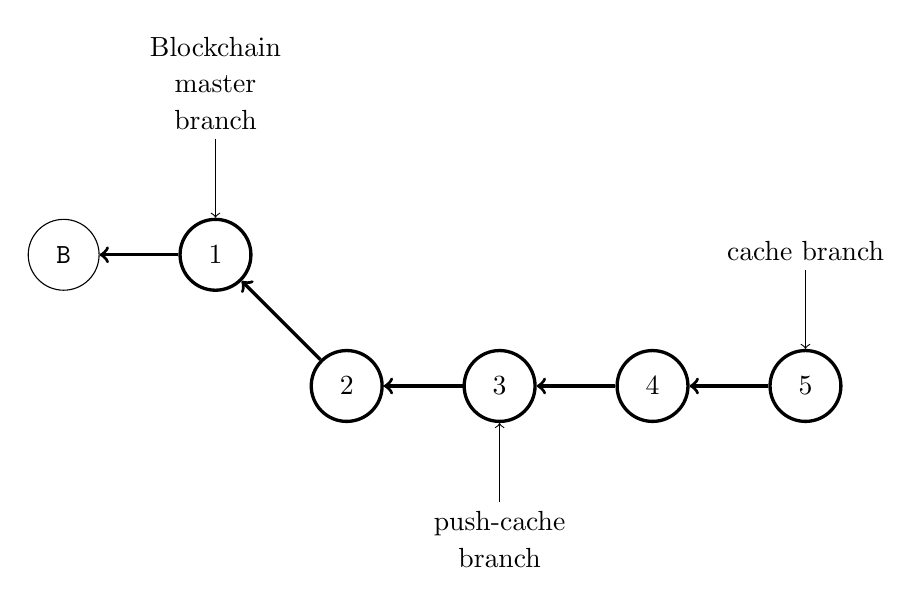
\begin{tikzpicture}[
			block/.style={circle, draw=black!100, very thick, minimum size=9mm},
			invis/.style={circle, draw=black!100, minimum size=9mm},
			label/.style={rectangle, text width=2cm, align=center}]                       
			\node[invis] (invis) {\texttt{B}};
			\node[block] (block1) [right=of invis] {1};
			\node[label] (labelmaster) [above=of block1] {Blockchain master branch};
			\node[block] (block2) [below right=of block1] {2};
			\node[block] (block3) [right=of block2] {3};
			\node[block] (block4) [right=of block3] {4};
			\node[label] (labelpushcache) [below=of block3] {push-cache branch};
			\node[block] (block5) [right=of block4] {5};
			\node[label] (labelcache) [above=of block5] {cache branch};
			\draw[->] (labelmaster.south) -- (block1.north);
			\draw[->] (labelpushcache.north) -- (block3.south);
			\draw[->] (labelcache.south) -- (block5.north);
			\begin{scope}[very thick, -stealth]
				\draw[<-] (invis.east) -- (block1.west);
				\draw[<-] (block1.south east) -- (block2.north west);
				\draw[<-] (block2.east) -- (block3.west);
				\draw[<-] (block3.east) -- (block4.west);
				\draw[<-] (block4.east) -- (block5.west);
			\end{scope}
		\end{tikzpicture}
		\caption{During push}
		\label{fig:replicaasync}
		\end{subfigure}	
		\begin{subfigure}[t]{\textwidth}
		\centering
		\begin{tikzpicture}[
			block/.style={circle, draw=black!100, very thick, minimum size=9mm},
			invis/.style={circle, draw=black!100, minimum size=9mm},
			label/.style={rectangle, text width=2cm, align=center}]                       
			\node[invis] (invis) {\texttt{B}};
			\node[block] (block1) [right=of invis] {1};
			\node[block] (block2) [right=of block1] {2};
			\node[block] (block3) [right=of block2] {3};
			\node[label] (labelmaster) [above=of block3] {Blockchain master branch};
			\node[block] (block4) [below right=of block3] {4};
			\node[label] (labelpushcache) [below=of block5] {push-cache branch};
			\node[block] (block5) [right=of block4] {5};
			\node[label] (labelcache) [above=of block5] {cache branch};
			\draw[->] (labelmaster.south) -- (block3.north);
			\draw[->] (labelpushcache.north) -- (block5.south);
			\draw[->] (labelcache.south) -- (block5.north);
			\begin{scope}[very thick, -stealth]
				\draw[<-] (invis.east) -- (block1.west);
				\draw[<-] (block1.east) -- (block2.west);
				\draw[<-] (block2.east) -- (block3.west);
				\draw[<-] (block3.south east) -- (block4.north west);
				\draw[<-] (block4.east) -- (block5.west);
			\end{scope}
		\end{tikzpicture}
		\caption{After push}
		\label{fig:replicaasyncfinished}
		\end{subfigure}	
		\caption{Blockchain data structure with cache for pushing to replicas}
	\end{figure}
	Figure \ref{fig:replicaasync} shows a blockchain with four transactions in the cache branch.
	Transactions 2 and 3 have been added to the push-cache by the push-thread and are in the process of being pushed to replicas. 
	Transactions 4 and 5, however, were added by the main thread after the push thread started its latest loop, and are therefore currently not being pushed to replicas.
	Figure \ref{fig:replicaasyncfinished} shows the state of the blockchain after the push thread has successfully pushed transactions 2 and 3 to a quorum of replicas.
	Now the master branch includes transactions 2 and 3, and the \textit{push-cache} branch has been updated to include transactions 4 and 5 will now be pushed to the blockchains of all the replicants.\\

	This new approach allows for the leader's functionality to be separated into two threads which can run in parallel. 
	This is beneficial because as two isolated threads, neither has a negative effect on the performance of the other.
	Whilst I implemented this approach in Logan, it suffered from race conditions caused by the coarse grained locking provided by Git and this has therefore not been included in the final implementation.
	Git's coarse grained locking meant that fake race conditions were being caused even though this approach does not add any true race conditions.
	A better library than Git with finer locking would allow the following mechanism to work without hindering the performance of the main leader thread.
	I am not aware of the existence of such a library so it would have to be built from scratch which would be outside the scope of this project.

	\section{Summary}
	In summary, in this chapter I detailed Logan's architecture and the data structure which it uses to store the blockchain and mempool.
	I then described the approach that Logan takes to achieving consensus and how this was inspired by my research into other popular consensus protocols.
	Finally I described how Logan implements passive replication to demonstrate how a more complex approach to fault tolerance may be implemented.

	\chapter{Evaluation}
	In this section I will describe my evaluation of Logan's performance.
	I will start by evaluating performance for the case where there is a single participant on the same machine as the leader. 
	I will then evaluate the cases where there is one and two participants on different machines to the leader.
	Finally I will evaluate the effect of replication on performance.\\

	\noindent In Section \ref{Consensus Requirements} I set out 5 success criteria which are summarised below in short. 
	\begin{itemize}
		\setlength{\itemindent}{2em}
		\item[\textbf{SC\_1}] Logan should achieve strict consistency
		\item[\textbf{SC\_2}] Logan should be able to achieve throughputs greater than 10tps
		\item[\textbf{SC\_3}] Logan should be able to achieve latencies of under a minute
		\item[\textbf{SC\_4}] Logan should achieve constant latencies in the size of the blockchain
		\item[\textbf{SC\_5}] Logan should have a scalable consensus mechanism 
	\end{itemize}
	Of these success criteria, the \nameref{Implementation} chapter shows how \textbf{SC\_1} is satisfied.
	In this chapter I will detail how Logan fulfils \textbf{SC\_2} and \textbf{SC\_3}.
	Lastly, I will show how Logan fails to achieve \textbf{SC\_4} and \textbf{SC\_5}, however, I will justify why this is not caused by my implementation.
	I will describe how a better synchronisation library would allow my implementation to achieve these goals.
	In this evaluation I have used a leader machine with a single core Intel Xeon 2.60GHz CPU, a 2.0MB cache and running Ubuntu 16.04.3 LTS. 
	My first participant machine has single core Intel Xeon 2.20GHz CPU with a 2.0MB cache and running Ubuntu 17.10.
	My second participant machine is a single core Intel Xeon 2.40GHz CPU with a 3.0MB cache and running Ubuntu 16.04.4 LTS.

	\subsection*{Metrics Used}
	In order to evaluate the performance of Logan, I have looked at three key metrics: latency, applied throughput and observed throughput.
	In this evaluation, I will define the latency of a transaction as the time elapsed between it being committed to a participant's mempool, and it being committed to the blockchain.
	In a blockchain system, it is important that the latency is as low as possible because latency dictates how long a user must wait before they can be sure of their transaction.
	In the context of a cryptocurrency, for example, long latencies will cause users to become irritated and potentially stop using the currency.
	Another useful measure is throughput, measured in transactions per second (tps), because it shows how well a system can cope with large loads.
	Specifically I will look at the \textit{applied} throughput which describes how frequently the participants are collectively making transactions, and the \textit{observed} throughput which describes how frequently the leader commits transactions to the blockchain.
	It is important that Logan should be able to achieve high observed throughputs because it is a limiting factor on how many users can interact with Logan at once.
	In my experiments I have control over applied throughput and I have measured the resulting observed throughput.
	I have also evaluated how the applied throughput affects latencies and lastly, I have looked at how latency varies with the size of the blockchain at different constant applied throughput.
	It is important that the system should be able to work well even when the size of the blockchain is large so that performance will not degrade over time.
	
	\section{Performance with a Local Participant}
	\subsection{Latency}
	Figure \ref{fig:locallatency} shows how the latency of Logan transactions varies as the size of the blockchain increases in the case that there is one participant on the same physical machine as the leader. 
	\begin{figure}
		\centering
		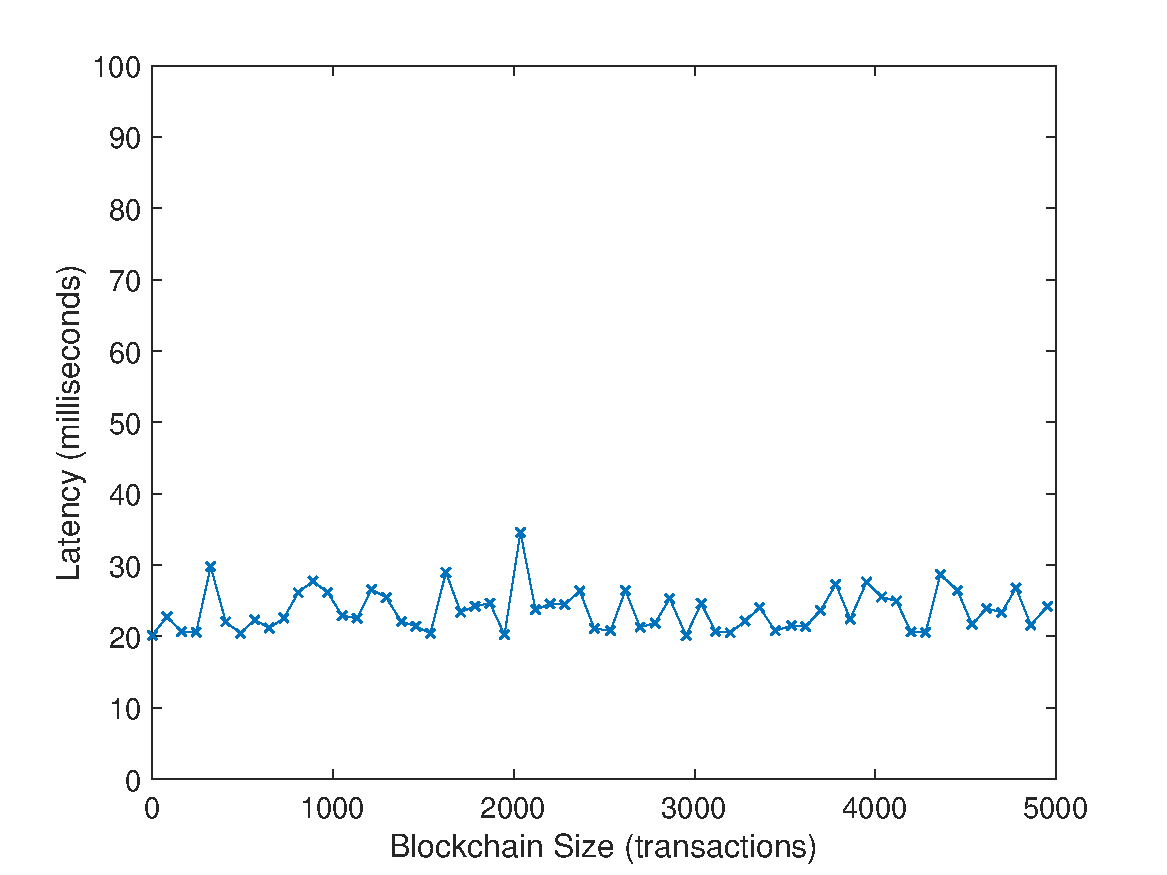
\includegraphics[width=0.8\textwidth, height=10cm]{figs/local_latency_vs_size.pdf}
		\caption{Latency variation with blockchain size on a local participant}
		\label{fig:locallatency}
	\end{figure}
	It is clear that the latency of adding a transaction is constant in the size of the blockchain.
	This is a very significant result because it proves that the logic which Logan uses is capable of achieving constant time blockchain appends in the size of the blockchain.
	This means that Logan achieves \textbf{SC\_4} for the case where there is a single local participant.
	Latencies are also very low, with an average of 25ms, which means that Logan also achieves \textbf{SC\_3}, in this use case.\\

	\subsection{Throughput}
	Now that I have evaluated latencies, I will look at the throughputs that the system is capable of achieving.
	Figure \ref{fig:singlocal} shows how the observed throughput varies with the applied throughput.  
	\begin{figure}
		\centering
		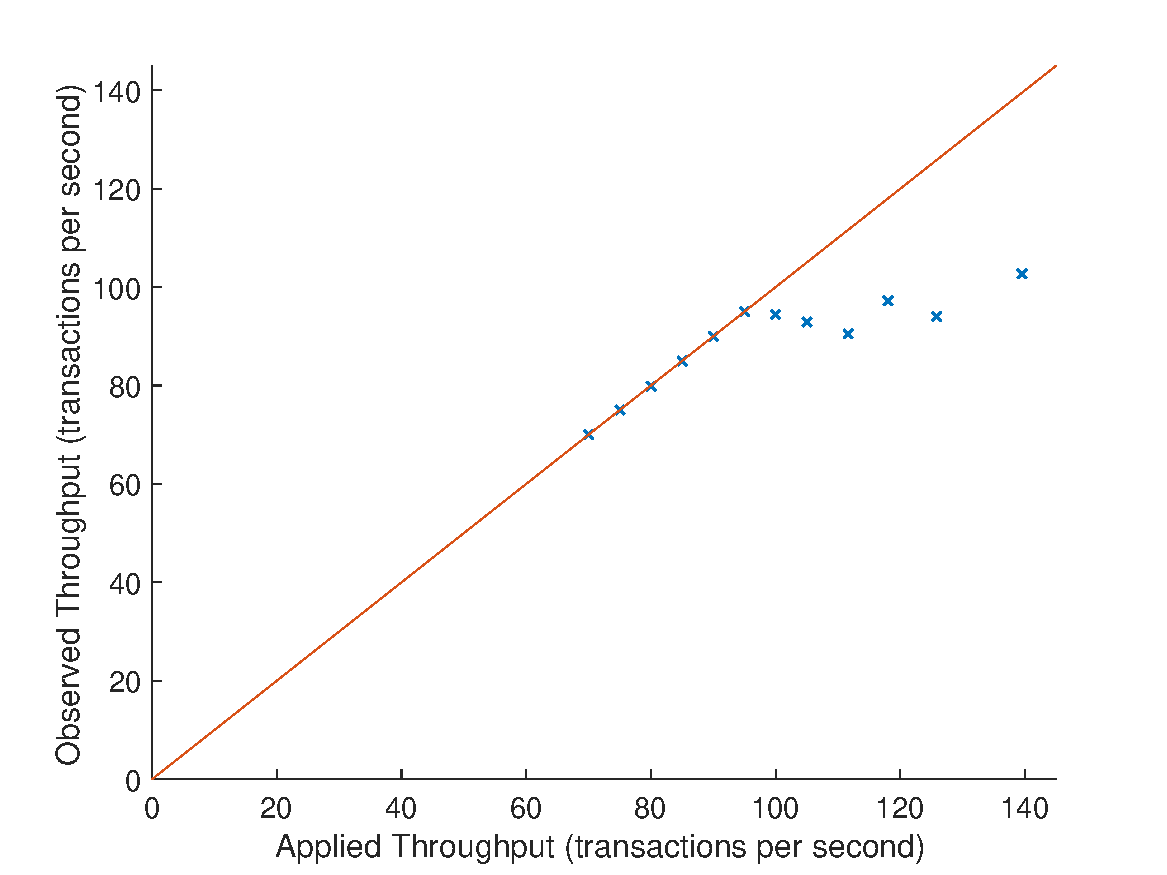
\includegraphics[width=0.8\textwidth]{figs/appliedvsobservedlocal.pdf} 
		\caption{Observed throughput with increasing applied throughput for a single local participant. Measurements have not been taken below an applied throughput of 50 transactions per second as it is assumed that observed throughput matches observed throughput for this range.}
		\label{fig:singlocal}
	\end{figure}
	The straight line plot in this figure indicates the performance of an ideal system that is capable of matching any applied throughput.
	The figure clearly shows that Logan is achieving ideal performance up until 100tps.
	At this point, the observed throughput starts to plateau as the system starts to become overloaded. 
	This result well exceeds the requirement of 10tps set out by \textbf{SC\_2} and shows that Logan's logic is capable of achieving high throughputs.
	It is worth noting that this result is using a relatively low performance virtual machine hosted in the cloud, with limited disk write performance. 
	It is reasonable to expect that a more powerful machine would be able to achieve significantly better results.\\

	\section{Performance with Single Remote Participant}
	\subsection{Latency}
	In order to see how the system performs when network latencies are involved, I first looked at Logan's performance when there is just one leader and one remote participant, i.e. a participant on a different machine to the leader.
	\begin{figure}
		\centering
		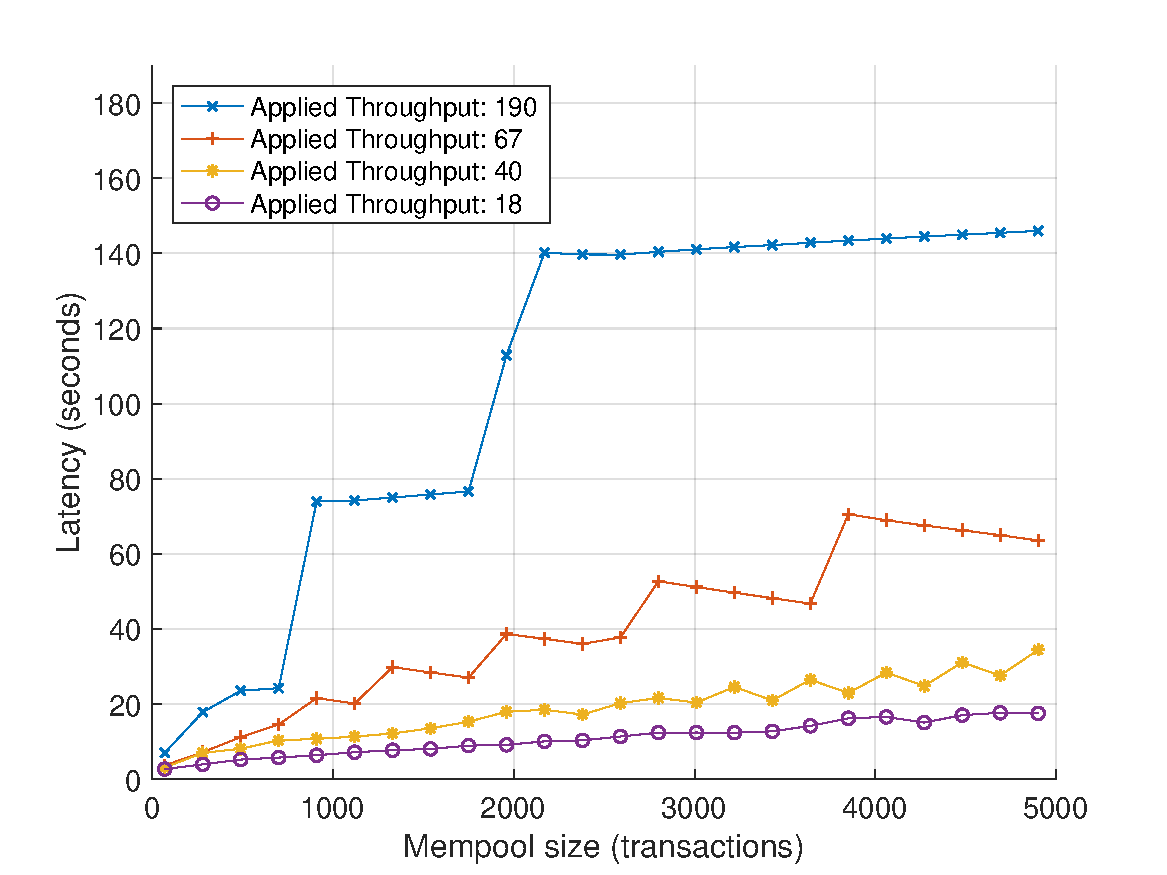
\includegraphics[width=0.8\textwidth]{figs/latencies_sizes_throughputs.pdf}
		\caption{Logan latencies with increasing blockchain size for one remote participant}
		\label{figs:remlatencysize}
	\end{figure} 
	Figure \ref{figs:remlatencysize} compares the latency of making a transaction and the size of the participant's mempool, for different applied throughputs.
	Mempool size has been used in place of blockchain size because it is the structure being pulled over the network, not the blockchain.
	The first noticeable feature of this graph is the saw-tooth shape of the latencies at high throughputs.
	In these cases, the flat or downward sloping segments represent transactions which were committed in the same poll cycle after being collectively retrieved over the network.
	Importantly, these teeth are relatively small up until around 40tps which suggests that this is roughly the throughput at which the system diverges from ideal performance.
	This figure also shows an obvious linear increase in latency for all throughputs except 190tps. 
	This plot is still linear although this trend is slightly obscured by the large size of the teeth in the sawtooth shape.
	These linear increases are undesirable behaviour as they indicate that large mempools will accompany poor performance.\\
	
	In order to examine what was causing the linear increase in latencies with mempool size, I logged the time that the leader spent completing the most time-consuming tasks for each poll cycle.
	These tasks turned out to be pulling mempool updates over the network and adding updates to the blockchain.
	Figure \ref{figs:leaderdelays} shows how these delays increase linearly over time and compares them with the number of updates that are pulled in each poll cycle.
	\begin{figure}
		\centering
		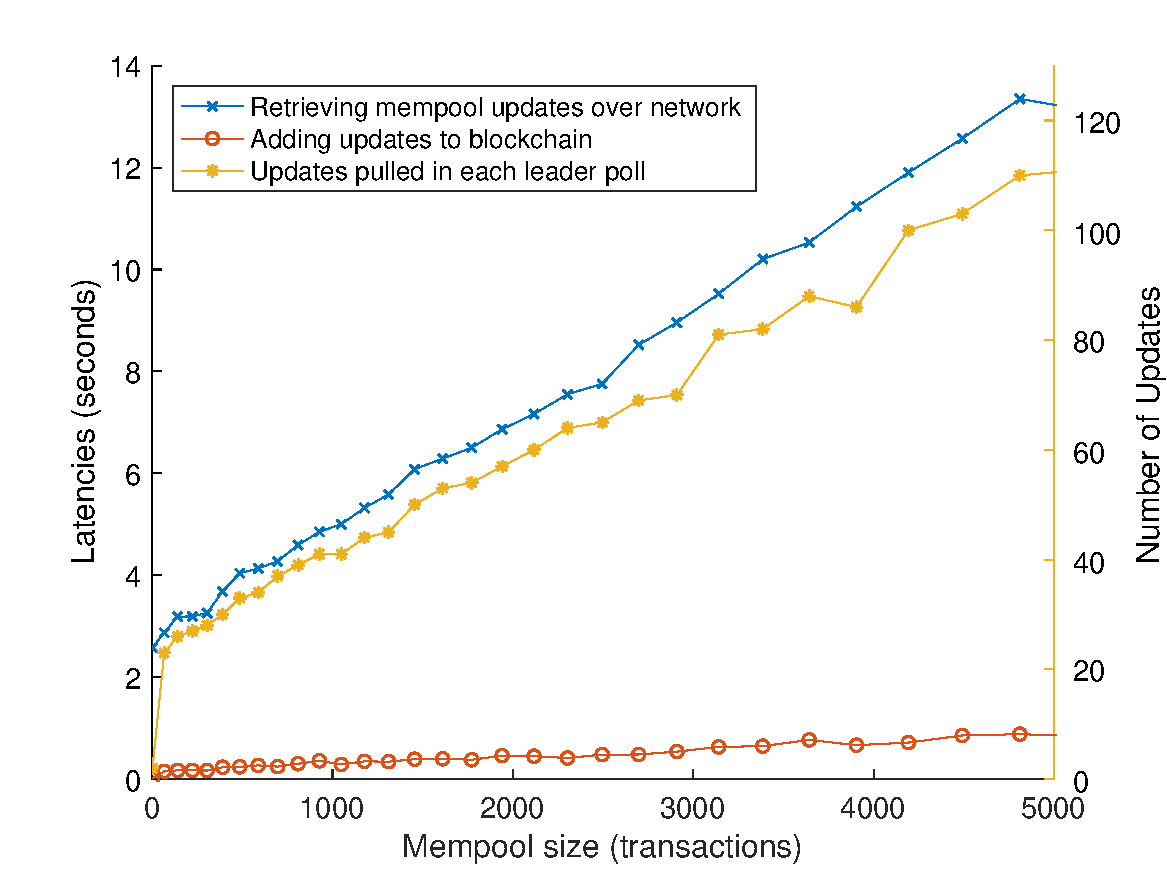
\includegraphics[width=0.8\textwidth]{figs/leader_delays_num_pulled.pdf}
		\caption{Delays incurred by leader for every poll cycle. Throughput is constant at 10tps}
		\label{figs:leaderdelays}
	\end{figure}
	The figure demonstrates a causality where an increase in time taken to pull mempool updates causes an increase the number of updates pulled in the next cycle. 
	This has the effect of increasing the time spent adding these updates to the blockchain.
	I can therefore conclude that the increase in the latency of pulling mempool updates prevents the system from being able to add transactions to the blockchain in constant time. \\

	\subsection{Using Pure Git}
	The latencies shown in Figure \ref{figs:leaderdelays} are particularly high. 
	This is because Irmin uses an OCaml implementation of Git called `OCaml Git' \parencite{OcamlGit}, and the performance of this implementation is much worse than the performance of `pure' Git \parencite{Git}, i.e. the implementation that is interacted with via a shell.
	I have created a modified implementation of Logan which calls pure Git commands directly rather than using OCaml Git.
	In this section I will show the extent to which this improves Logan's performance.
	This approach comes with many disadvantages such as worse compatibility with unikernel systems and a lack of type checking.
	I am not suggesting that this is an adequate solution, but I am showing that a better Git implementation in OCaml can drastically improve performance.\\ 

	\begin{figure} 
		\centering
		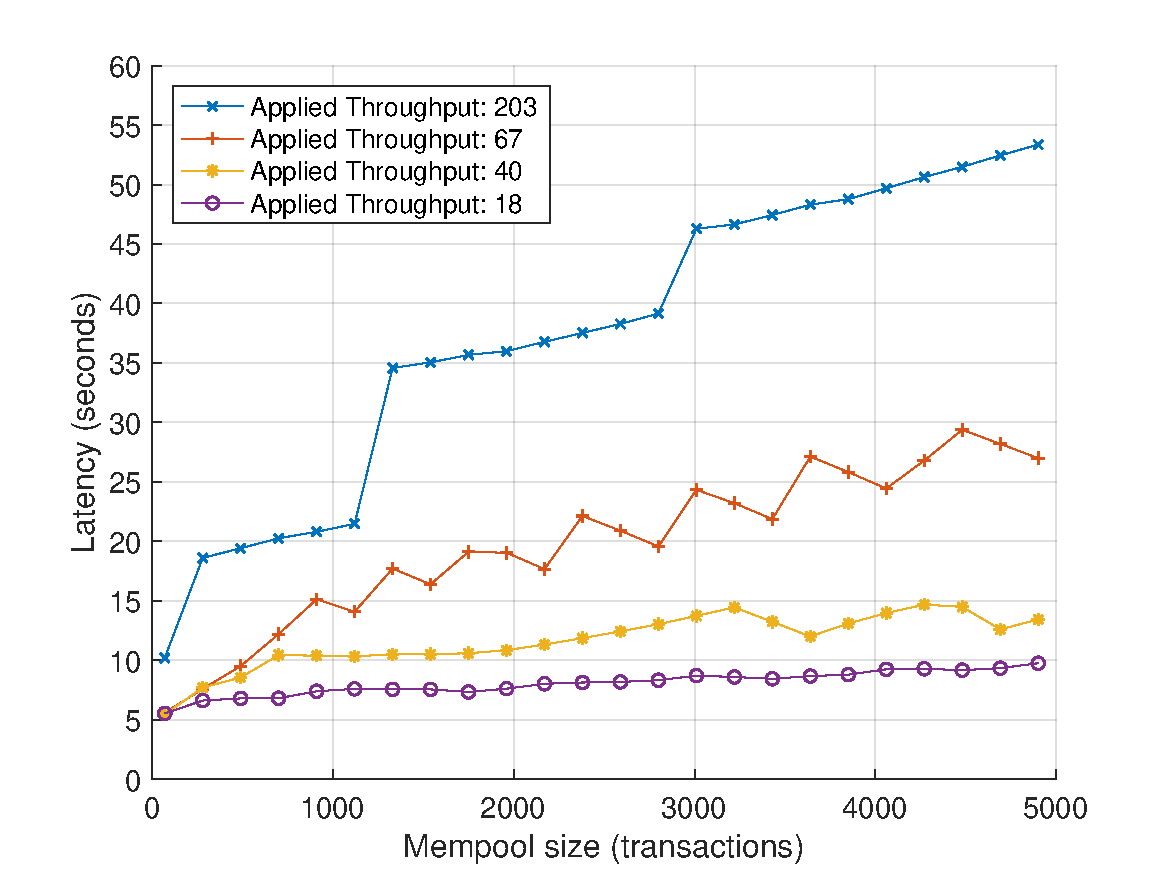
\includegraphics[width=0.8\textwidth]{figs/latency_sizes_throughputs.pdf}
		\caption{Logan latencies with increasing blockchain size for one remote participant. Leader is using pure Git}
		\label{figs:latenciespuregit}
	\end{figure}
	Figure \ref{figs:latenciespuregit} is a parallel of Figure \ref{figs:remlatencysize} but using this new implementation instead. 
	The figure shows that the system can perform significantly better by using pure Git. 
	Specifically, the system can achieve much better constant factors in the increase of latencies with mempool size.
	For an applied throughput of 10tps, latencies rise from 2.7s to 15s with OCaml Git. 
	For this new implementation using pure Git latencies rise from 5.5s to 8s. 
	So whilst the latencies are initially larger, they have much better constant factors using pure Git.
	\begin{figure}
		\centering
		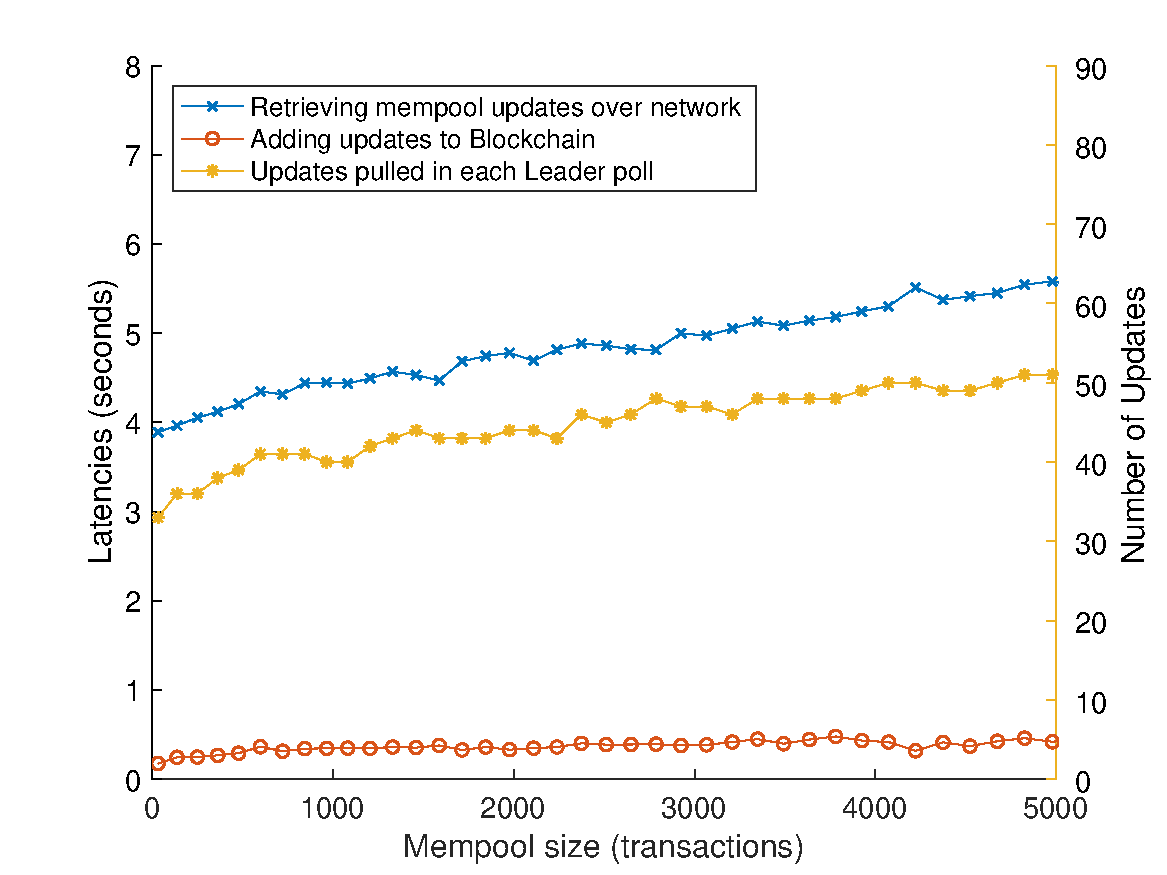
\includegraphics[width=0.8\textwidth]{figs/bottlenecks.pdf}
		\caption{Delays incurred by leader for every poll cycle when using pure Git. Throughput is constant at 10tps}
		\label{figs:bottleneckspuregit}
	\end{figure}
	Figure \ref{figs:bottleneckspuregit} is a parallel of Figure \ref{figs:leaderdelays} that demonstrates that this speedup is due to the greatly reduced times that the leader spends pulling mempool updates as the mempool size grows.
	Whilst this bottleneck is much lower than before, it still takes up much more time than any other stage of the leader's execution.
	This suggests that Git is still a very inefficient way of transferring updates to the leader.  
	This could be due to many unnecessary overheads in the implementation of Git, such as the mechanism Git uses for finding new updates to be transferred between repositories. 
	Therefore if a better protocol was used, even better performance could be achieved.
	I am not aware of an implementation of a better protocol in OCaml so this would have to be built from scratch which is out of the scope of this project.\\

	\subsection{Throughput}
	In the previous sections, I have evaluated how transaction latencies evolve over time, and compared the results for different applied throughputs.
	This does not, however, shed light on when the system reaches its maximum throughput capacity.
	\begin{figure}
		\centering
		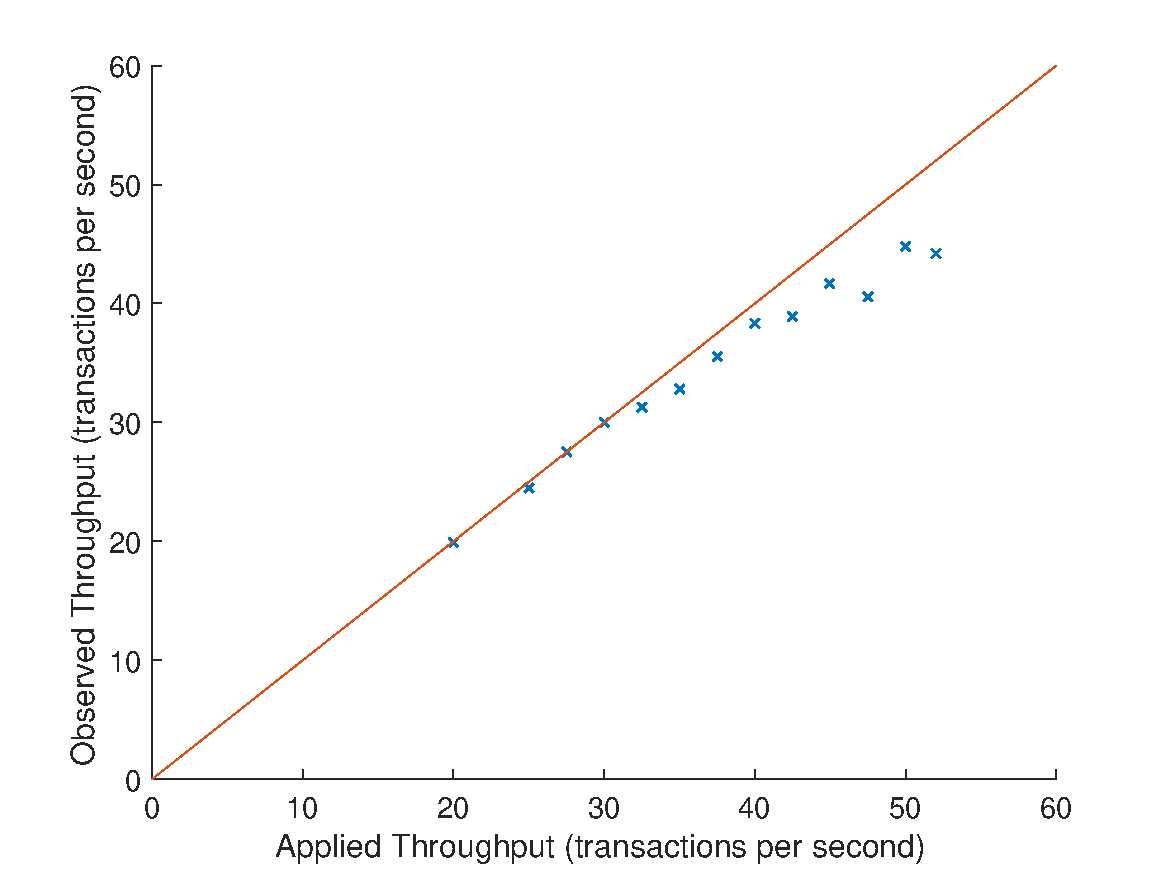
\includegraphics[width=0.8\textwidth] {figs/appliedvsobservedsingle.pdf}
		\caption{Observed throughput with increasing applied throughput for a single remote participant using pure Git. Measurements have not been taken below an applied throughput of 20tps as it is assumed that observed throughput matches observed throughput for this range.}
		\label{figs:appliedobservedsingle}
	\end{figure}
	Figure \ref{figs:appliedobservedsingle} shows how observed throughput varies with applied throughput. 
	This is again compared to a linear plot showing the ideal performance of a leader that never becomes overloaded.
	This figure shows that the system starts diverging from ideal performance at an applied throughput of around 30tps.
	Whilst the performance gets worse, it does not plateau and the observed throughput never actually decreases.
	This is because the participant is not capable of committing enough transactions to overload the leader in this scenario.
	Overall, this result demonstrates that an ideal sustained operating throughput is around 20tps which satisfies \textbf{SC\_2}.
	Although the system will be able to handle bursts of higher throughputs, it will not be able to cope with these throughputs for sustained periods of time.

	\subsection{Achieving Constant Time Latencies}\label{sect:bettersync}
	I have now shown that Logan can perform well by using pure Git, however, there is still the unfortunate result that transaction latencies increase linearly with the size of the mempool being pulled.
	This is due to the linear increase shown by Figure \ref{figs:bottleneckspuregit} and the fact that Logan's mempools are always growing. 
	There are two ways of solving this problem which I will detail in this section.\\

	The first approach requires a better synchronisation mechanism that allows updates to be pulled with constant time in the size of the mempool.
	This could be achieved by using, for instance, a streaming protocol that keeps track of all the updates which have previously been sent, rather than re-evaluating all the updates that need to be sent every time a pull operation is made. 
	This protocol would allow a leader to pull updates in constant time (assuming constant applied throughput), which would in turn mean that the time taken for adding blocks to the blockchain would be constant.
	This means that all the leader's operations could be completed in constant time and therefore latencies would be constant in the size of the mempool/blockchain. \\

	Another approach would be to use a queue rather than a log for the mempool data structures. 
	The fact that mempools are always growing is not a requirement for Logan.
	A mempool only needs to contain the latest uncommitted transactions and therefore a queue data structure would be a natural choice.
	In this scenario, participants would add transactions to their mempool queue which would then be pulled and popped by the leader.
	Participants could periodically merge changes (which are just pops) from the leader's copy in order to reduce the size of their mempool.
	This would mean that the size of the mempool would not be linear in the number of transactions made by a participant, and would no longer cause a linear increase in the time taken by a leader to pull updates.
	This would also have the desirable side effect of allowing the participant to see when the leader has recognised requested transactions, because they would get popped off the queue. 
	Whilst Ezirmin provides a queue data structure, I have not used it in this project because I anticipated that many of the bugs I encountered with Ezirmin logs would also exist for Ezirmin queues.
	Additionally, because of the bidirectional nature of merging changes (i.e. popping and pushing), it would not be trivial to use command line Git in this case. \\

	Overall, in the case of a single remote participant, Logan is able to comfortably reach throughputs of up to 30tps which is above the requirement of 10tps set out by \textbf{SC\_2}. 
	Latencies in this case are initially less than 10s which is a good result for most applications and fulfils \textbf{SC\_3}.
	Finally, whilst Logan does not fulfil \textbf{SC\_4}, I have demonstrated how this is due to the overheads from using Git, and I have shown two methods that would allow Logan to achieve this goal.

	\section{Performance with Multiple Remote Participants}
	\subsection{Latency}
	I have shown that Logan can perform well with a single remote participant, but it remains to show how this performance scales to multiple participants. 
	Figure \ref{figs:tworems} shows how the latency of making transactions varies with throughput when the pure Git protocol is used with two remote participants.
	\begin{figure}
		\centering
		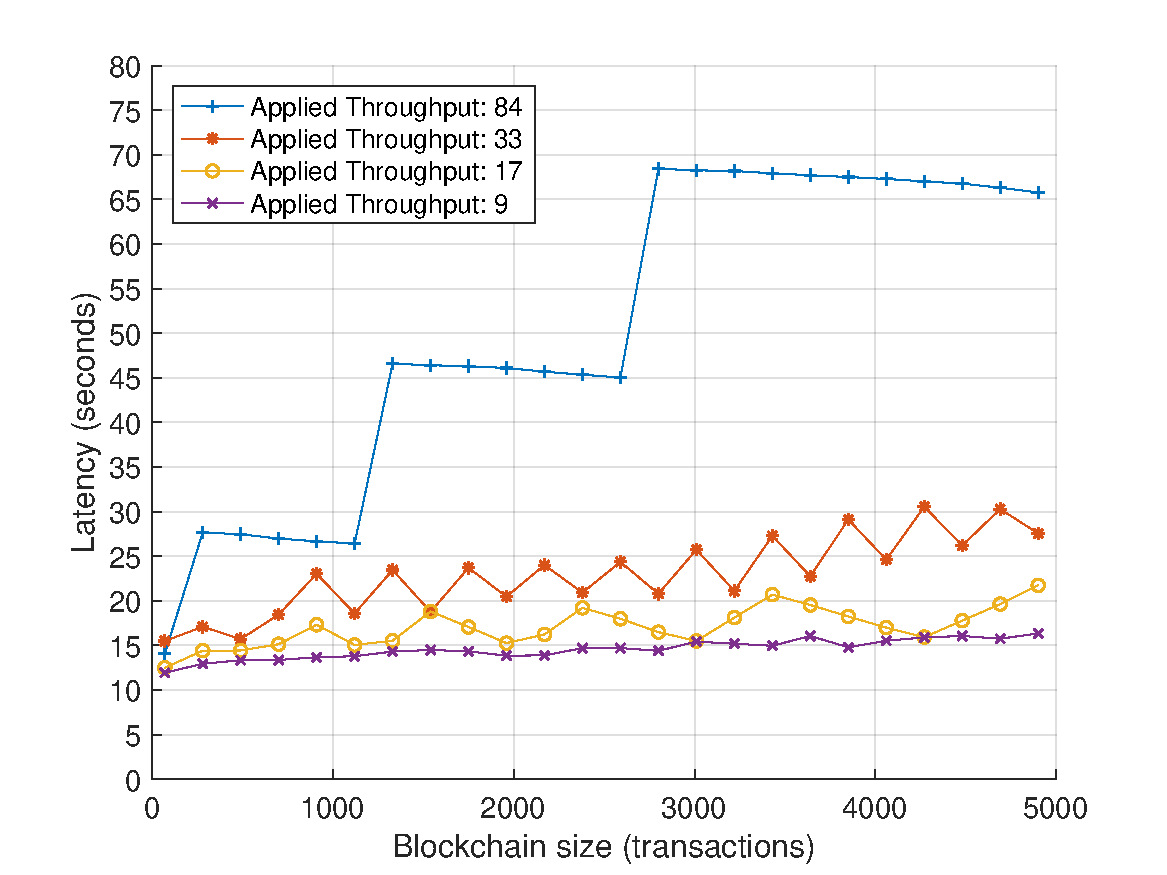
\includegraphics[width=0.8\textwidth]{figs/2latencies_sizes_throughputs.pdf}
		\caption{Logan latencies with increasing blockchain size for two remote participants.}
		\label{figs:tworems}
	\end{figure}
	For a throughput of around 10tps, transaction latencies will rise by 4.5s over 5000 transactions compared to 3.1s in the single participant case.
	I consider this a modest increase that would indeed be solved by using a better synchronisation protocol as described in Section \ref{sect:bettersync}. 
	With this protocol, Logan would satisfy \textbf{SC\_4}.\\

	Another difference to the case with only a single remote participant is the fact that transaction latencies now start at 11.9s, whereas they were 5.5s in the single participant case.
	This is because native Git does not allow any parallelism when pulling updates from multiple different remote repositories, and therefore, all remote repositories must be pulled sequentially.
	Even if a protocol is used that can achieve constant time blockchain appends, this result limits latencies to be linear in the number of remote nodes in a network which is undesirable. 
	Indeed, using the OCaml Git implementation shows a similar increase of initial transaction latency from 2.7s to 4.5s.
	It is unfortunate that neither OCaml Git nor pure Git are able to exploit more levels of IO parallelism, because it is not unreasonable to expect that these implementations should be able to handle concurrent pulls into isolated branches. 
	Should this be possible, the latencies would only increase by a modest amount with the number of participants and Logan would be able to achieve \textbf{SC\_5}.\\

	Overall I conclude that Logan does not satisfy \textbf{SC\_4} or \textbf{SC\_5}, but a synchronisation mechanism should allow these goals to be reached. 
	However, even with multiple nodes in a network, latencies will still be modest in comparison to the 10 minute latency of a Bitcoin transaction, so even in its current state I can consider my implementation to be somewhat successful.

	\subsection{Throughput}
	Finally I will evaluate Logan's throughput performance for two remote participants.
	Figure \ref{figs:tworemthrthr} shows the observed throughput against the applied throughput of a Logan system with two participants and one leader.
	\begin{figure}
		\centering
		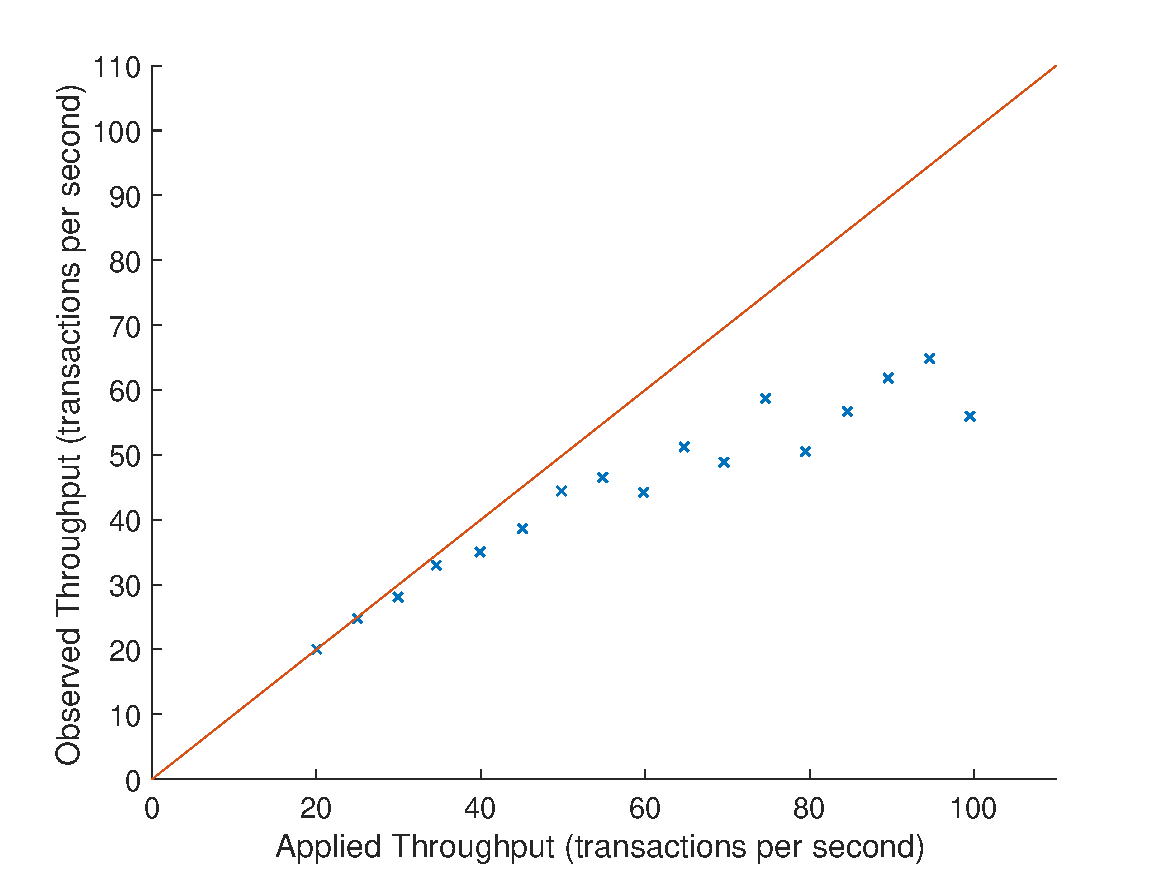
\includegraphics[width=0.8\textwidth]{figs/appliedvsobserved2r.pdf}
		\caption{Observed throughput with increasing applied throughput for two remote participants using pure Git. Measurements have not been taken below an applied throughput of 20tps as it is assumed that observed throughput matches observed throughput for this range.}
		\label{figs:tworemthrthr}
	\end{figure}
	The system starts to diverge from ideal throughput at around 30tps, indicating that a suitable sustained operating throughput would be around 20tps.
	Again, it can be seen that the system can cope with higher applied throughputs for short bursts  but not for sustained periods of time. 
	This is exactly the same as the case for only a single remote participant. 
	Whilst in the previous section, I showed that the latencies will grow with the number of nodes in a network, this result shows that a system will still be able to cope with the same throughputs. 
	In this sense, not only does Logan satisfy \textbf{SC\_2}, but also \textbf{SC\_5}.

	\section{Performance with Leader Replication}
	In Section \ref{sec:faulttol} I described how Logan can be updated to introduce the simple notion of a passive replica. 
	In order to justify that this only introduces minor latencies, I have tested the performance of the system with one remote participant at a throughput of 10tps. 
	Figure \ref{figs:confirmationtimes}  shows the time taken between a transaction being added to the blockchain's cache branch, and it being merged into the blockchain's main branch, i.e. after being pushed to a replica.
	\begin{figure}
		\centering
		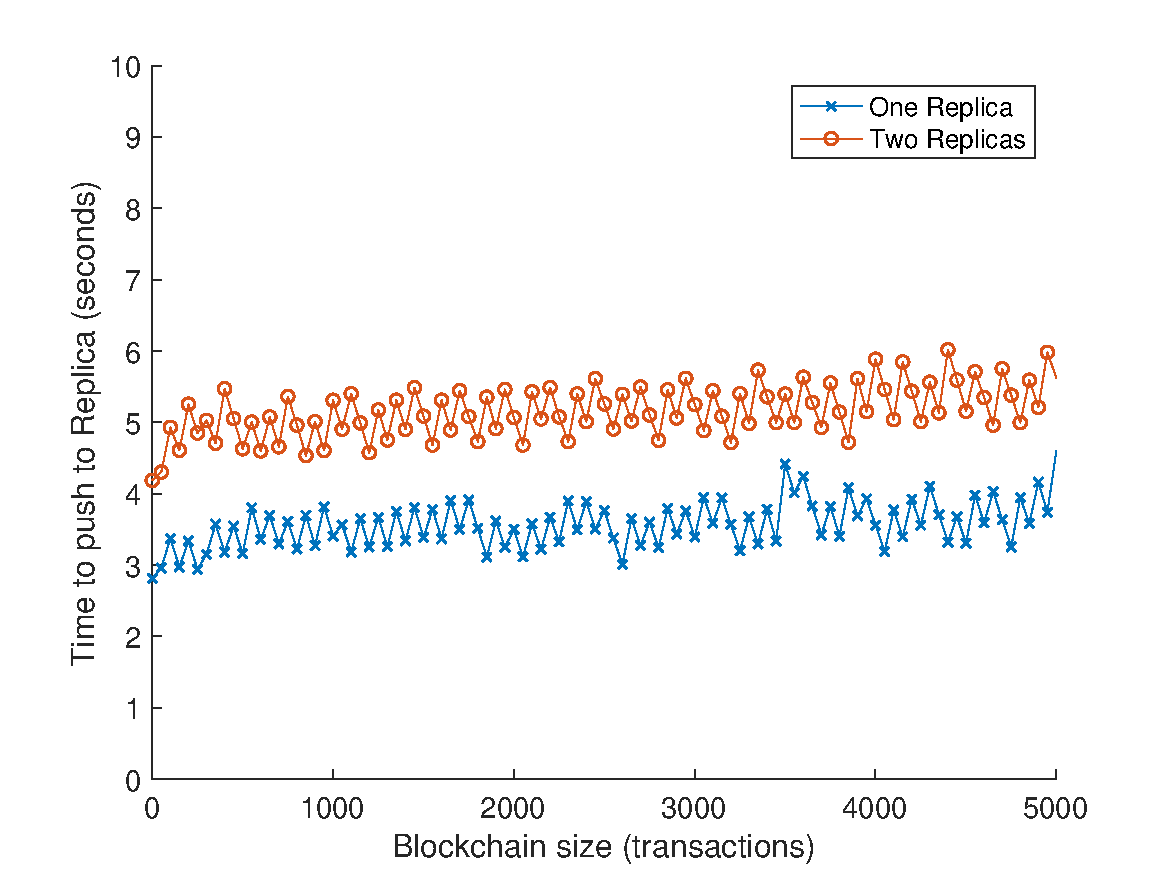
\includegraphics[width=0.8\textwidth]{figs/confirmationlatencies.pdf}
		\caption{Time taken between transactions being added to cache branch and being merged to main blockchain branch, for a single remote replica}
		\label{figs:confirmationtimes}
	\end{figure}
	Unfortunately the latencies of pushing to a remote repository also increase with the size of the blockchain, as is the case for pulling.
	However, this is again a problem that is minor and would not exist with a better synchronisation protocol. 
	Importantly, for the case where there is one replica, the additional latencies are around 3s which is small and would be an acceptable waiting time for most applications.
	In this case, the system's latencies are still well within the requirements of \textbf{SC\_3}.
	Figure \ref{figs:confirmationtimes} also shows that using two replicas rather than one increases latencies by roughly 1.5s. 
	I again conclude that this is a very acceptable latency in the context of \textbf{SC\_3}.\\

	Additionally if Logan were to implement my suggested approach of using a daemon thread to push transactions to replicas, there would be no additional latencies to the leader's loop cycle and this means that it should in theory be able to sustain exactly the same throughputs as it would without having any replicas.
	I therefore consider this a successful demonstration of passive replication and a good starting point for developing a more complex fault tolerance solution.

	\section{Summary}
	In summary, in this section I have demonstrated how Logan can perform well with a single participant on the same machine as the leader. 
	I have then shown how this performance scales to the situations with both one and two remote participants. 
	Throughput of the system scales well although latencies grow linearly in the size of the blockchain and I have attributed this to the implementation of Git used by Logan.
	I have motivated how a better synchronisation protocol would allow my implementation to achieve all its success criteria. 
	Finally, I have shown that the effect of replication on the system is only modest, and I have shown how my approach to replication can be modified to have no effect on the main leader thread.

	\chapter{Conclusion}
	\section{Successes}
	When I started this project, my goals were to design a library that would allow developers to easily create blockchain applications using OCaml.
	I have designed and implemented Logan, a blockchain library that achieves that goal.
	Logan uses a leader based approach for consensus and can achieve latencies of around 10s and throughputs of up to 30tps.
	Logan uses Git to store data and to communicate over the network and this has proved to be a large bottleneck in this project. 
	Latencies are linear in the size of the blockchain if there are multiple nodes in a network and this is due to Git's coarse grained locking.
	However, I have shown that Git is the only bottleneck in Logan's operation and that a better synchronisation protocol would allow linear blockchain appends and very reasonable latencies. 

	\section{Possible Further Work}
	There are many different ways in which Logan could be improved in the future.
	Here are some of the most important parts which could be improved:
	\begin{itemize}
	\item \textbf{Improved Synchronisation Protocol}.
	The biggest flaw with Logan that I have mentioned in this report is the use of Git.
	Further work on Logan should include a new implementation of the network synchronisation protocol.
	\item \textbf{Failure Tolerance and Changing Leaders}.
	Tolerating failure is an aspect of this project that I have only touched upon in this project. 
	I have shown how Logan can perform passive replication but further work could include implementing an automated approach for detecting and recovering from failure. 
	This work could also include allowing a system to reallocate a leader after leader failure.
	\item \textbf{Adding Participants Dynamically}.
	Currently, as well as only being able to define a single leader, participants can only be defined statically. 
	Some consensus mechanisms introduce ways of adding and removing nodes to a network and I think it would be very feasible to build this feature into Logan.
	\end{itemize}

	%%%%%%%%%%%%%%%%%%%%%%%%%%%%%%%%%%%%%%%%%%%%%%%%%%%%%%%%%%%%%%%%%%%%%
	% the bibliography
	\printbibliography
	\addcontentsline{toc}{chapter}{Bibliography}
	
	%%%%%%%%%%%%%%%%%%%%%%%%%%%%%%%%%%%%%%%%%%%%%%%%%%%%%%%%%%%%%%%%%%%%%
	% the appendices
	\appendix

	\chapter{Project Proposal}
	
	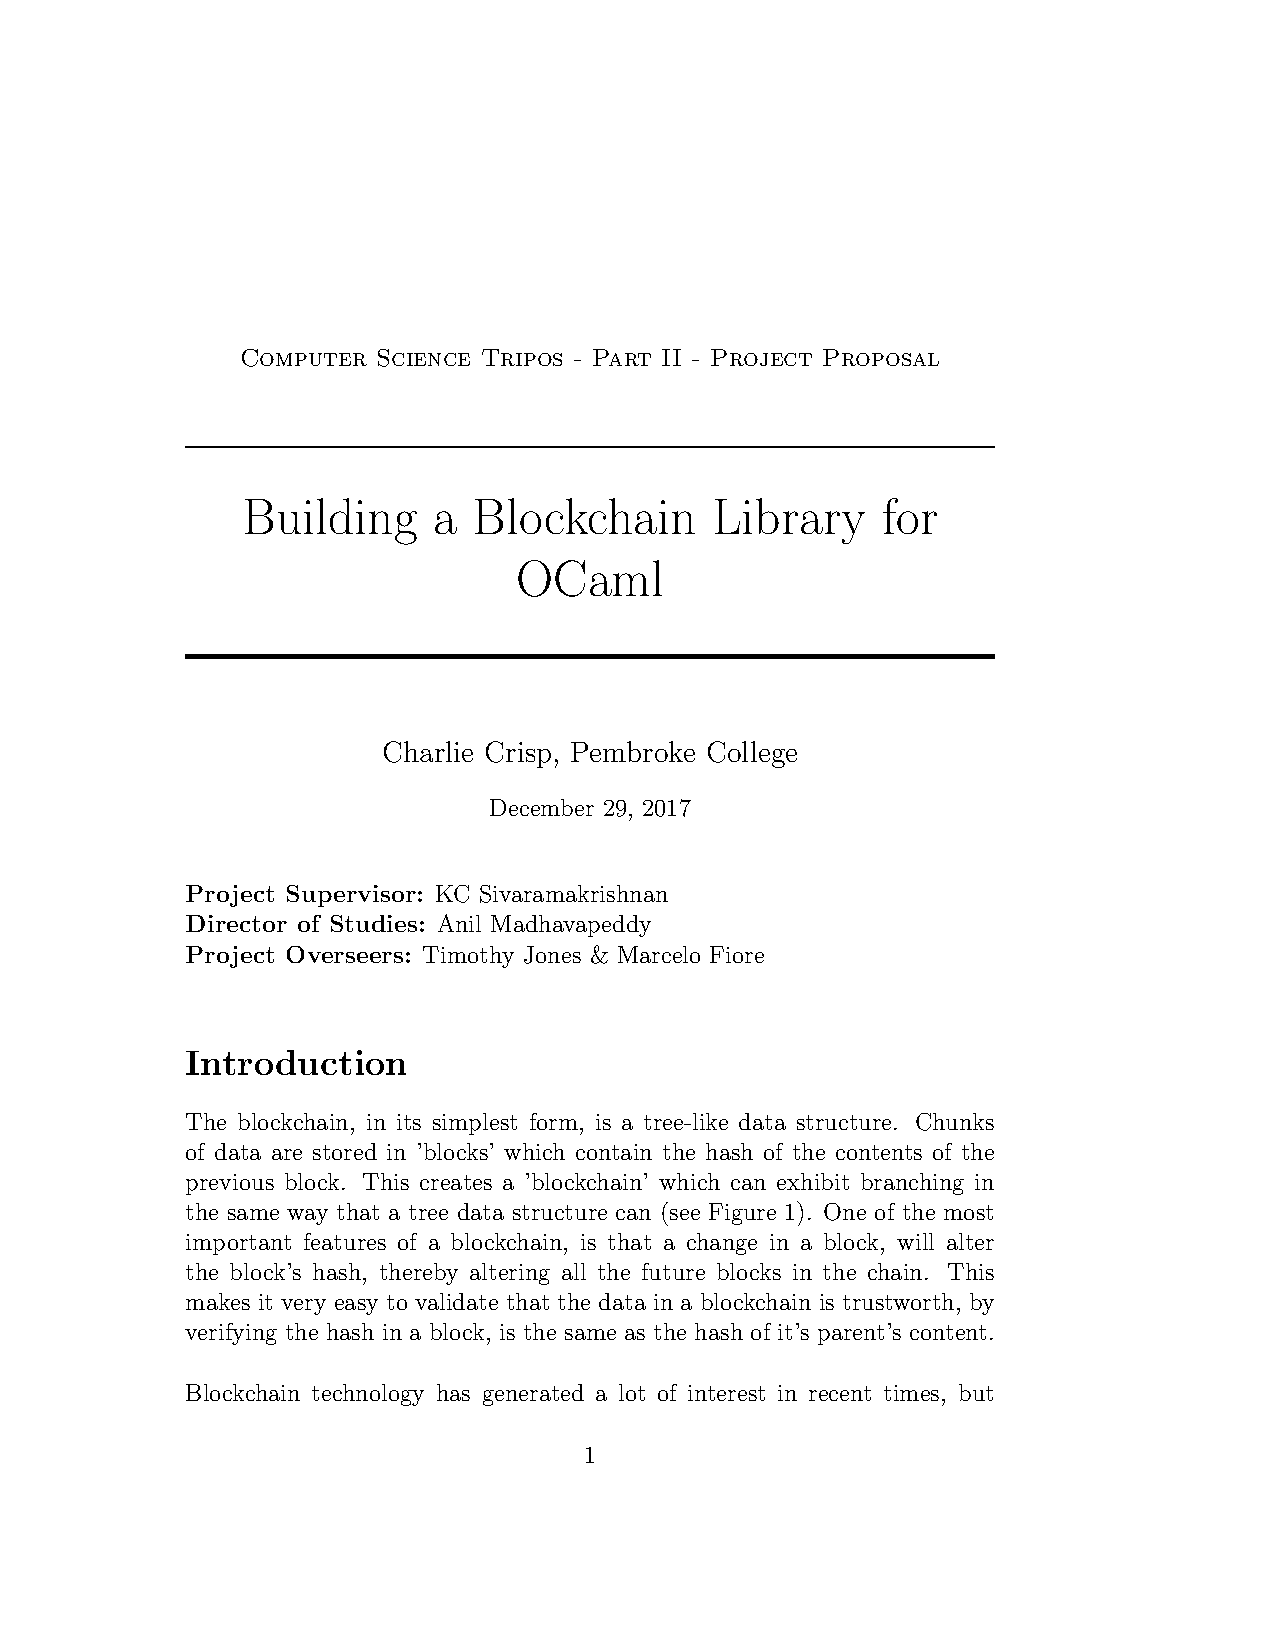
\includepdf[pages=-]{Part_II_Project_Proposal_Draft.pdf}
	
	\end{document}